
% Chapter 

%\chapter{Quantitative Analysis of Thesis reflexivity}{Analyse de la réflexivité} % Chapter title

\bpar{
\chapter{Reflexive Analysis}
}{
\chapter{Analyse réflexive}
}


\bpar{
\markboth{\thechapter\space Reflexivity}{\thechapter\space Reflexivity}
}{
\markboth{\thechapter\space Réflexivité}{\thechapter\space Réflexivité}
}


\label{app:reflexivity} % For referencing the chapter elsewhere, use \autoref{ch:name} 

%----------------------------------------------------------------------------------------


\bpar{
We have throughout all this work the crucial role of a reflexivity in the research process. It has played a role for the definition of objects or questions asked, in a concrete way in works directly based on fieldwork, or in the elaboration of theories with a recursive aspect. Without pretending having exhaustively constructed a ``meta-viewpoint'' as recommended by~\cite{morin1991methode} for the construction of a complex thinking, we suggest to have brought preliminary elements of answer. 
}{
Nous avons vu tout au long de ce travail le rôle crucial d'une réflexivité dans la démarche de recherche. Celle-ci a pu jouer pour la définitions des objets ou les questions posées, concrètement dans les travaux directement basés sur un travail de terrain, ou dans l'élaboration de théories ayant un aspect récursif. Sans prétendre avoir exhaustivement construit un ``méta-point de vue'' comme préconisé par~\cite{morin1991methode} pour la construction d'une pensée complexe, nous suggérons avoir apporté des éléments de réponse de manière préliminaire.
}


\bpar{
We propose here, as a ``meta-conclusion'', to proceed to a quantitative analysis for reflexivity, by applying the methods we developed to our work itself. We do in a first part the analysis of the scientific landscape from the corpus of our bibliography, and then analyze in a second part the evolution of the knowledge produced in terms of projects and of knowledge domains.
}{
Nous proposons ici, en guise de ``méta-conclusion'', de mener une analyse quantitative pour la réflexivité, en appliquant les méthodes développées à notre travail lui-même. Nous menons dans un premier temps l'analyse du paysage scientifique à partir du corpus de notre bibliographie, puis analysons dans un second temps l'évolution de la connaissance produite en termes de projets et de domaines de connaissance.
}


\bpar{
This approach is particularly original since to the best of our knowledge there exist no monograph explicitly including its own analysis using quantitative tools. We defend a more systematic use of such approaches, to foster the development of a knowledge at the second order.
}{
Cette démarche est particulièrement originale puisqu'il n'existe à notre connaissance pas de monographie incluant explicitement sa propre analyse par des outils quantitatifs. Nous prenons le parti d'une utilisation plus systématique de ce genre de démarche, pour encourager le développement d'une connaissance de second ordre.
}


%%%%%%%%%%%%
\section{Hypernetwork analysis}{Analyse par hyperréseau}


\bpar{
We apply here the methodology using citation and semantic networks developed in Chapter~\ref{ch:modelinginteractions}. The initial corpus is constituted by all our bibliography\footnote{Fixed at the 27/11/2017, and available at \url{https://github.com/JusteRaimbault/CityNetwork/raw/master/Models/Reflexivity/data/CityNetwork_20171127.bib}.} which includes 834 references.
}{
Nous appliquons ici la méthodologie par réseau de citation et réseau sémantique développée en Chapitre~\ref{ch:modelinginteractions}. Le corpus initial est constitué de l'ensemble de notre bibliographie\footnote{Figée au 27/11/2017, et disponible à \url{https://github.com/JusteRaimbault/CityNetwork/raw/master/Models/Reflexivity/data/CityNetwork_20171127.bib}.} qui comporte 834 références.
}


\subsection{Citation Network}{Réseau de citation}


\bpar{
We reconstruct the citation network at depth two from this initial corpus, and obtain a consequent network ($\left|V\right| = 177428$, $\left|E\right| = 203317$), of average degree $2.29$ (average in-degree $1.15$). The core of the network, constituted by vertices with a degree larger than or equal to 2 for the largest connected component (which covers 98\% of the network), has a size of $\left|V\right| = 19714$ and $\left|E\right| = 47348$.
}{
Nous reconstruisons le réseau de citation à profondeur deux à partir de ce corpus initial, et obtenons un réseau conséquent ($\left|V\right| = 177428$, $\left|E\right| = 203317$), de degré moyen $2.29$ (degré moyen entrant $1.15$). Le coeur du réseau, constitué des sommets de degré supérieur ou égal à 2 pour la plus grande composante connexe (qui couvre 98\% du réseau), est de taille $\left|V\right| = 19714$ et $\left|E\right| = 47348$.
}


% IGRAPH 9dd0bbb DN-- 177428 203317
% mean(degree(citation))
%[1] 2.291825
% mean(degree(citation,mode="in"))
% [1] 1.145913

% citationcore
%IGRAPH c617c58 DN-- 19714 47348 -- 


\bpar{
A detection of communities using the Louvain algorithm gives a directed modularity of 0.74 for 19 communities with a size larger than 10. We interpret the communities by the tags given in Table~\ref{tab:app:reflexivity:citationcoms}. We recover domains that are directly covered and used in our work (Urban Systems, Spatial Models of Urban Growth), and other neighbors mentioned but not directly used (Fractals, Economic Geography, Space Syntax).
}{
Une détection de communautés par algorithme de Louvain donne une modularité dirigée de 0.74 pour 19 communautés de taille supérieure à 10. Nous interprétons les communautés par les étiquettes données en Table~\ref{tab:app:reflexivity:citationcoms}. Nous retrouvons des domaines directement couverts et utilisés dans notre travail (Systèmes Urbains, Modèles Spatiaux de Croissance Urbaine), et d'autres voisins évoqués mais pas directement utilisés (Fractales, Economie Géographique, Space Syntax).
}



%Chaos, Economie Géographique, Systèmes Urbains, ABM, Datamining, Réseaux, Statistiques Spatiales, Fractales, Lois Puissance, Economie Géographique Évolutionnaire, Epistémologie Quantitative, Modèles de Croissance Urbaine Spatialisés, Complexité, LUTI, Physique des Villes, Données Spatio-temporelles, Réseaux Biologiques, Space Syntax, VGI.




%%%%%%%%%%%%%
\begin{table}
\apptabcaption{\textbf{Citation communities.} The size of communities is given as a proportion of the size of the core of the network.\label{tab:app:reflexivity:citationcoms}}{\textbf{Communautés de citation.} La taille des communautés est donnée en proportion de la taille du coeur du réseau.\label{tab:app:reflexivity:citationcoms}}
\begin{tabular}{|l|l|}
\hline
\bpar{
Community & Size \\ \hline
}{
Communauté & Taille \\ \hline
}
Economic Geography & 12.4 \% \\
Power Laws & 9.1 \% \\
Networks & 7.92 \% \\
Spatial Urban Growth Models & 7.67 \% \\
Physics of Cities & 7.43 \% \\
ABM & 7.37 \% \\
Complexity & 7.19 \% \\
LUTI & 7.16 \% \\
Urban Systems & 5.15 \% \\
Spatial Statistics & 5.13 \% \\
Evolutionary Economic Geography & 5.03 \% \\
Spatio-temporal data & 3.18 \% \\
Datamining & 2.81 \% \\
Quantitative Epistemology & 2.43 \% \\
Space Syntax/Procedural modeling & 2.43 \% \\
Fractals & 2.02 \% \\
VGI & 1.8 \% \\
Biological Networks & 1.33 \% \\
Chaos & 0.624 \% \\\hline
\end{tabular}
\end{table}
%%%%%%%%%%%%


%%%%%%%%%%%%
\begin{figure}
	%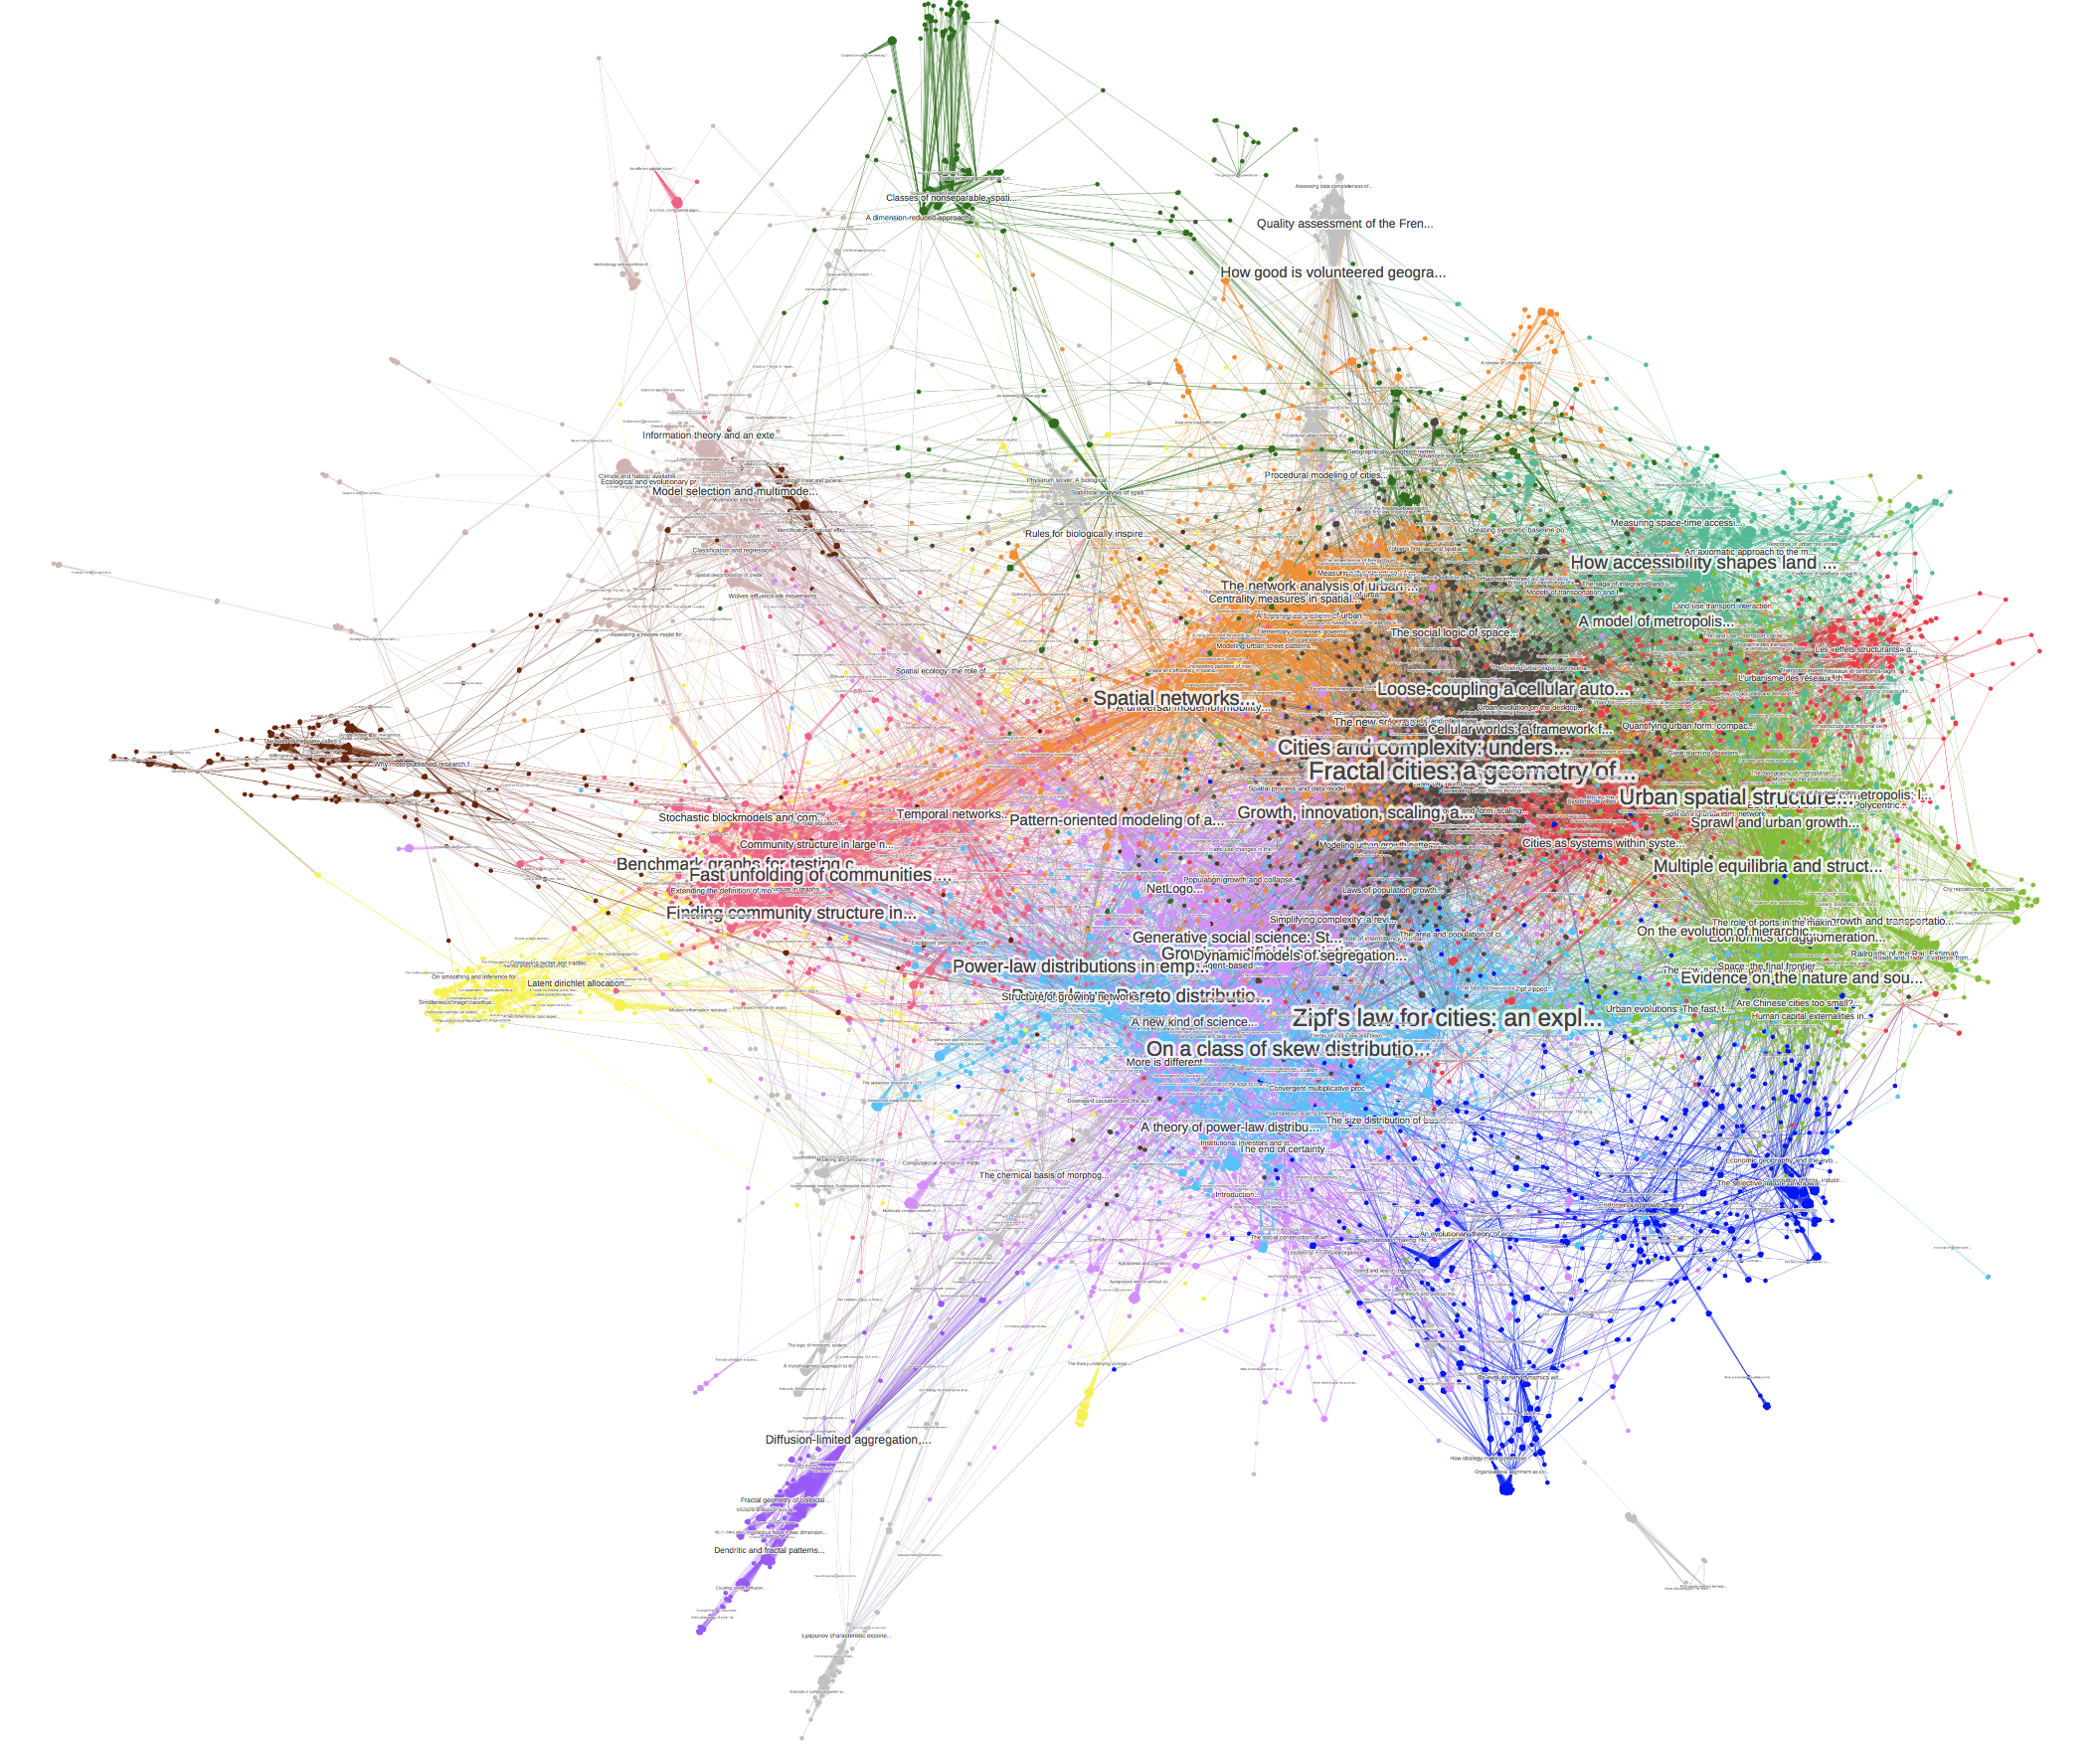
\includegraphics[width=\textwidth]{Figures/Reflexivity/citcore.png}
	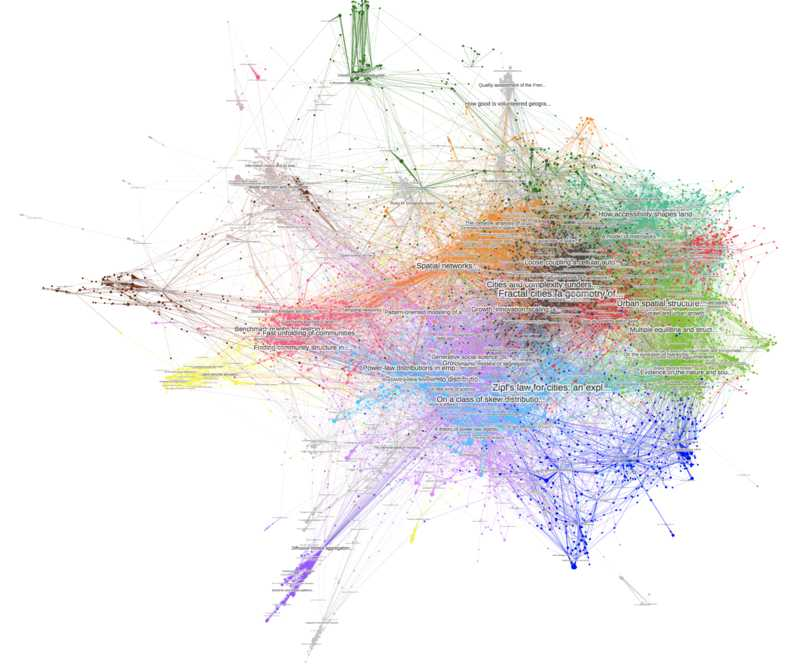
\includegraphics[width=\linewidth]{Figures/Final/F-reflexivity-citnw.jpg}
	\appcaption{\textbf{Citation network.} We visualize only the core of the network, constituted here by nodes with a degree larger than or equal to 2. The network is spatialized with the algorithm Force Atlas 2. The size of labels is proportional to the degree of nodes, and the color gives the community.\label{fig:app:reflexivity:citnw}}{\textbf{Réseau de citation.} Nous visualisons uniquement le coeur du réseau, constitué ici des noeuds de degré supérieur ou égal à 2. Le réseau est spatialisé par algorithme Force Atlas 2. La taille des labels est proportionnelle au degré des noeuds, et la couleur donne la communauté.\label{fig:app:reflexivity:citnw}}
\end{figure}
%%%%%%%%%%%%

\bpar{
The citation network is visualized in Fig.~\ref{fig:app:reflexivity:citnw}. The position of communities is very instructive to situate our work, which forms bridges between different domains depending on the viewpoint chosen. If we take the point of view of urban systems, the corresponding community (in red) makes a bridge between LUTI models (turquoise) and urban growth models (black) on one side, and economic geography on the other side (in green). If we take the viewpoint of simulation models (ABM community, purple), the link is established between Power Laws (light blue) and networks and spatial networks (magenta and orange). Auxiliary communities are attached at the periphery: Quantitative Epistemology (yellow) is close to network analysis, whereas the analysis of spatio-temporal processes (dark green) is relatively independent. Communities within which our models can be thematically classified (growth models and urban systems) are located at the core of the compact part of the network: this confirms that the direction explored are not auxiliary, and that all principal auxiliary domains evoked where ``necessary'' in the sense of a strong connection between communities here.
}{
Le réseau de citation est visualisé en Fig.~\ref{fig:app:reflexivity:citnw}. Le positionnement des communautés est très instructif pour situer notre travail, qui forme des ponts entre différents domaines selon le point de vue choisi. Si nous prenons le parti des systèmes urbains, la communauté correspondante (en rouge) fait le pont entre modèles LUTI (turquoise) et modèles de croissance urbaine (noir) d'une part, et économie géographique (en vert). Si on se place du point de vue des modèles de simulation (communauté ABM, violet), le lien est fait entre Lois Puissances (bleu clair) et les réseaux et réseaux spatiaux (magenta et orange). Des communautés annexes se rattachent à la périphérie : Epistémologie Quantitative (jaune) est proche de l'analyse de réseau, tandis que l'analyse des processus spatio-temporels (vert foncé) est relativement indépendante. Les communautés dans lesquelles nos modèles peuvent être classifiés de manière thématique (modèles de croissance et systèmes urbains) sont situées au coeur de la partie compacte du réseau : cela confirme que les directions explorées ne sont pas périphériques, et que l'ensemble des domaines principaux périphériques évoqués étaient ``nécessaires'' au sens d'une forte connexion entre communautés ici.
}



%%%%%%%%%%%%
\subsection{Semantic network}{Réseau sémantique}

% kminopt=0;kmaxopt=500;freqminopt=0;freqmaxopt=10000;ethopt=5


\bpar{
After collecting the abstracts, we obtain 91412 references on which it is possible to proceed to the semantic analysis. The construction of the raw co-occurrences network, after filtering links with a weight smaller than 5, and for a number of keywords $K_W = 50000$, yields a semantic network with $\left|E\right|\simeq 16\cdot 10^6$. The sensitivity analysis to filtering parameters suggests to choose $k_{min} = 0$, $k_{max}=500$, $f_{max} = 10000$, $\theta_w = 5$, what produces a semantic network of size $\left|V\right| = 37482$ and $\left|E\right| = 218926$, with 26 communities and a modularity of $0.78$. Main communities can be labeled as: toxicology, chemistry, political sciences, theoretical ecology, urban systems, sustainability, innovation economics, spatial analysis, physiology, physics, networks, bio-anthropology, health, statistics, microbiology, transportation, biological networks, health geography, botany, evolution, ecology, genetics.
}{
Après collecte des résumés, nous obtenons 91412 références sur lesquelles il est possible de procéder à l'analyse sémantique. La construction du réseau de co-occurrences brut, en filtrant les liens de poids inférieur à 5, et pour un nombre de mots-clés $K_W = 50000$, donne un réseau sémantique avec $\left|E\right|\simeq 16\cdot 10^6$. L'analyse de sensibilité aux paramètres de filtrage nous suggère de choisir $k_{min} = 0$, $k_{max}=500$, $f_{max} = 10000$, $\theta_w = 5$, ce qui fournit un réseau sémantique de taille $\left|V\right| = 37482$ et $\left|E\right| = 218926$, avec 26 communautés et une modularité de $0.78$. Les communautés principales peuvent être labellisées comme : toxicologie, chimie, sciences politiques, écologie théorique, systèmes urbains, soutenabilité, économie de l'innovation, analyse spatiale, physiologie, physique, réseaux, bio-anthropologie, santé, statistiques, microbiologie, transports, réseaux biologiques, géographie de la santé, botanique, évolution, écologie, génétique.
}


% 'toxicology','chemistry','political science','theoretical ecology','urban systems (french)','sustainibility','innovation economics','maup','physiology','NA','physics', 'networks','bioanthropology','health','statistics','microbiology', 'transportation','biological network','copyrights','publication','health geography','botanics','evolution','ecology','formulas','genetics')


\bpar{
It is less evident to use this typology to understand our work, in comparison with the citation network, since remote domains (toxicology, chemistry, physiology, botany) can be found in relatively small amount in our citation corpus (coming from common citations on morphogenesis or ecology for example) but form then communities that are particularly isolated in the semantic network. We give in Fig.~\ref{fig:app:reflexivity:interdisc} the distribution of semantic interdisciplinarities for each citation community. At the exception of evolutionary economic geography which is relatively flat (and thus rather closed) and voluntary geographical information (VGI) which exhibits a peak at 0 (which is expected for such a specific domain), citation communities have fundamentally the same interdisciplinarity profile.
}{
Il est moins évident d'utiliser ce découpage pour comprendre notre travail, en comparaison au réseau de citation, puisque des domaines lointains (toxicologie, chimie, physiologie, botanique) se retrouvent en nombre relativement faible dans notre corpus de citation (provenant de citations communes sur la morphogenèse ou l'écologie par exemple) mais forment ensuite des communautés particulièrement isolées dans le réseau sémantique. Nous donnons en Fig.~\ref{fig:app:reflexivity:interdisc} la distribution des interdisciplinarités sémantiques par communautés de citation. À l'exception de l'économie géographique évolutionnaire qui est relativement plate (et donc assez cloisonnée) et de l'information géographique volontaire (VGI) qui présente un pic à 0 (attendu d'un domaine si spécifique), les communautés de citation ont fondamentalement le même profil d'interdisciplinarité.
}


%%%%%%%%%%%%
\begin{figure}
	%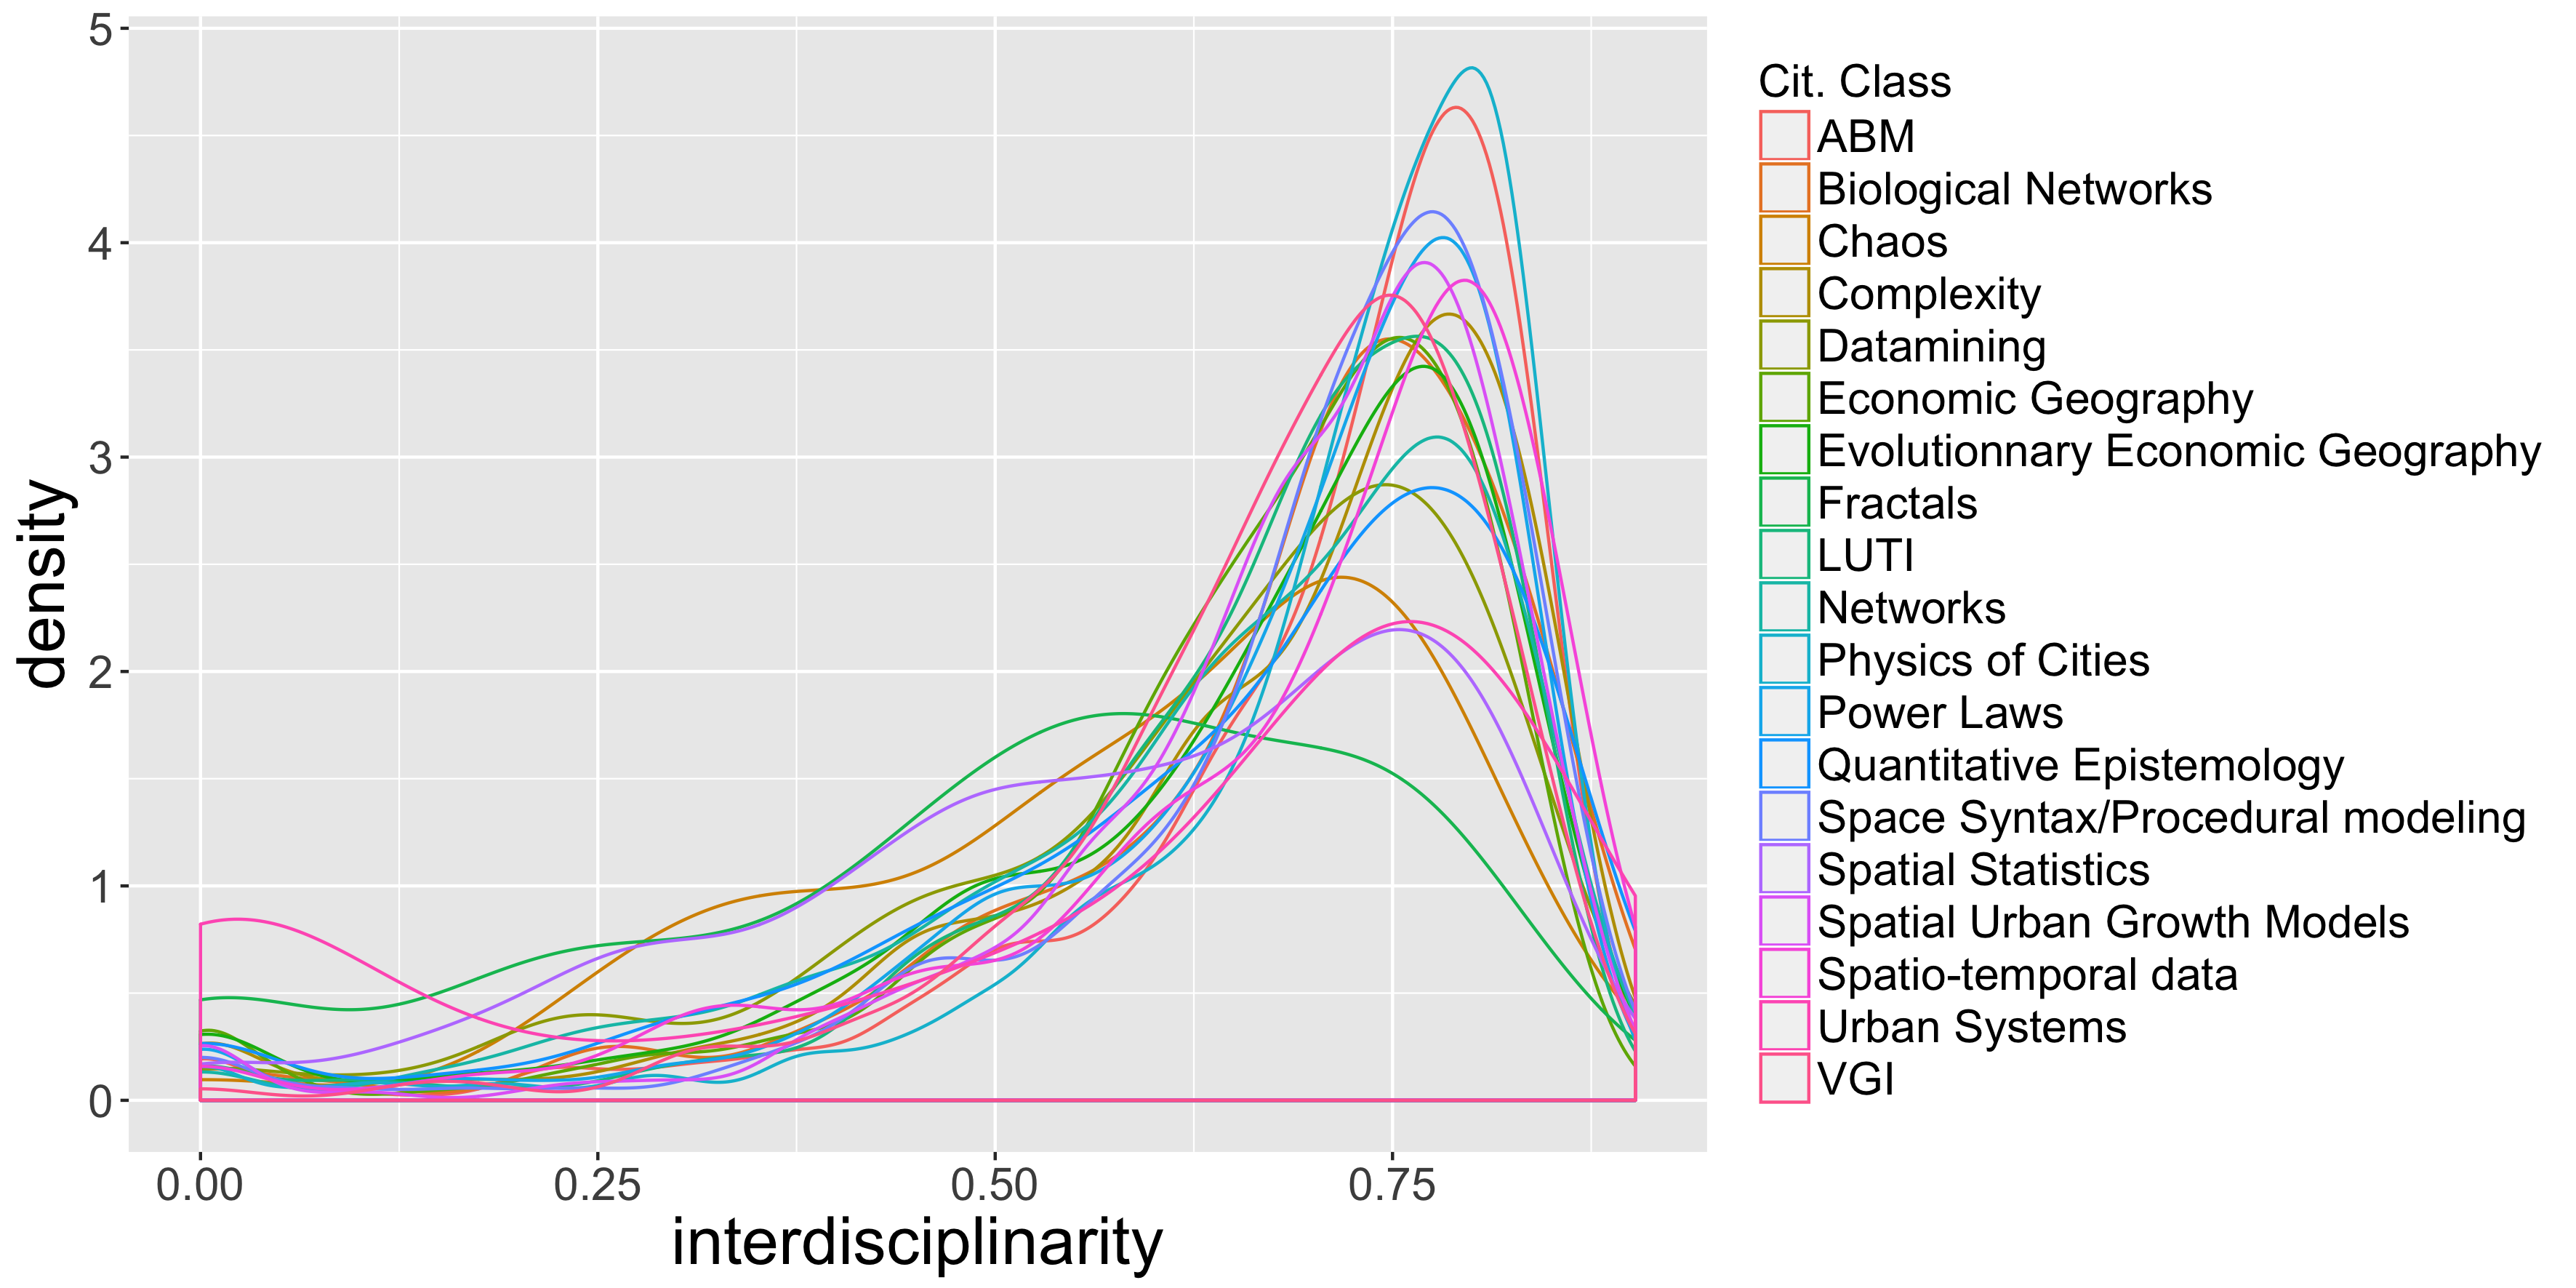
\includegraphics[width=\linewidth]{Figures/Reflexivity/interdisciplinarities.png}
	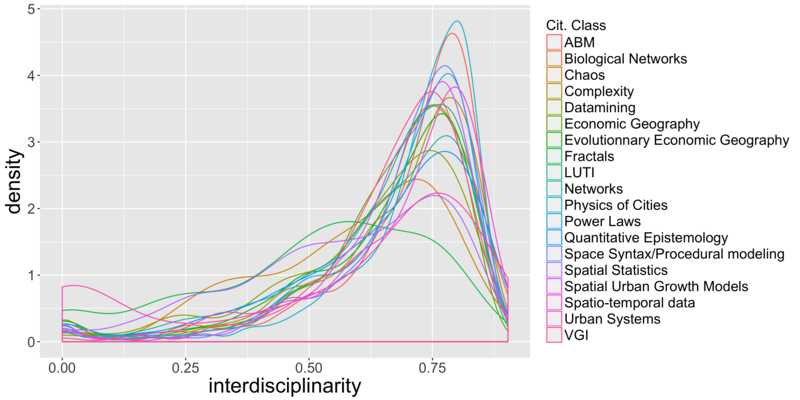
\includegraphics[width=\linewidth]{Figures/Final/F-reflexivity-interdisc.jpg}
	\appcaption{\textbf{Distribution of interdisciplinarities for each citation community.}\label{fig:app:reflexivity:interdisc}}{\textbf{Distribution des interdisciplinarités par communauté de citation.}\label{fig:app:reflexivity:interdisc}}
\end{figure}
%%%%%%%%%%%%








%%%%%%%%%%%%
\section{Interaction between projects}{Interaction entre projets}


\bpar{
We propose here to quantify the evolution of the different projects and of their interactions, and also of associated knowledge domains. A table of the time spent on each project, with a precision of half an hour, has been held between the 16/02/2015 and the 16/02/2018\footnote{It is available at \url{https://github.com/JusteRaimbault/CityNetwork/raw/master/Docs/Organisation/Projects.ods}. For the analyses here, we use the version frozen at the 02/12/2017.}. A project is defined as a minimal consistent entity, either by its thematic (for example: morphogenesis model of~\ref{sec:densitygeneration}) either by its content (case studies, geographical theory). These have been defined progressively in time, and some overlap or are the precursors of others: we have thus built a classification a posteriori under the form of ``macro-projects'' which globally correspond to the final articulation. We also associate to them a main knowledge domain\footnote{Knowing that there is a non-negligible bias in the fact of attributing a unique domain to a project, since domains are generally intimately linked at the core of knowledge production itself. The constraint of data collection however leads to this segmentation which is relatively reductionist.} and the main section of this memoir to which they are attached.
}{
Nous proposons ici de quantifier l'évolution des différents projets et de leur interactions, ainsi que des domaines de connaissance associés. Un tableau du temps passé sur chaque projet, à la demi-heure près, a été tenu entre le 16/02/2015 et le 16/02/2018\footnote{Celui-ci est disponible à \url{https://github.com/JusteRaimbault/CityNetwork/raw/master/Docs/Organisation/Projects.ods}. Pour les analyses ici, nous utilisons la version figée au 02/12/2017.}. Un projet est défini comme une entité minimale cohérente, soit par sa thématique (par exemple : modèle de morphogenèse de~\ref{sec:densitygeneration}) soit par son contenu (cas d'études, théorie géographique). Ceux-ci ayant été défini au cours du temps, certains se recoupent ou sont précurseurs d'autres : nous leur avons donc associé une classification a posteriori sous forme de ``macro-projets'' qui correspondent globalement à l'articulation finale. Nous leur attribuons également un domaine de connaissance majoritaire\footnote{Tout en sachant qu'il existe un biais non-négligeable dans le fait d'attribuer un domaine unique à un projet, puisque les domaines sont généralement intimement liés au coeur même de la production de connaissance. La contrainte de captation des données pousse toutefois à cette segmentation relativement réductionniste.} et la section principale de ce mémoire auxquels ils se rattachent.
}


\bpar{
The list of projects is given in Table~\ref{tab:app:reflexivity:projects}, with the macro-project, the knowledge domain and the cumulated time. The Fig.~\ref{fig:app:reflexivity:time} gives the temporal distribution according to these different modalities, in time. We confirm a non-linear organization, most of projects and chapters being treated in parallel. For example, the chapter~\ref{ch:mesocoevolution} has been the object of a first preliminary exploration in the first months, and a resurgence when converging as the intellectual maturity had been acquired. Methods regularly punctuate the distribution, but culminate just before the first half. Modeling projects, similarly to empirical studies, are also regularly distributed, whereas the conceptual takes more time in the end, what confirms that it necessitates the other domains and a thorough reflection. 
}{
La liste des projets est donnée en Table~\ref{tab:app:reflexivity:projects}, avec le macro-projet, le domaine et connaissance et le temps cumulé. La Fig.~\ref{fig:app:reflexivity:time} donne la répartition temporelle selon ces différentes modalités, dans le temps. Nous confirmons une organisation non-linéaire, la plupart des projets et chapitres étant menés en parallèle. Par exemple, le chapitre~\ref{ch:mesocoevolution} a fait l'objet d'une première exploration préliminaire dans les premiers mois, puis une résurgence à la convergence lorsque la maturité intellectuelle a été acquise. Les méthodes ponctuent régulièrement la répartition, mais culminent juste avant la première moitié. Les projets de modélisation, comme l'empirique, sont également régulièrement répartis, tandis que le conceptuel prend plus de place à la fin, ce qui confirme que celui-ci nécessite les autres domaines et une réflexion approfondie.
}


%%%%%%%%%%%%%
\begin{table}
	\apptabcaption{\textbf{Description of projects.} The section links to the part of the memoir where the project is mainly used. Global generic tasks are not taken into account in the chapter cumulated count (Memoire: writing of this memoir; Academic: academic life; Bibliography: general readings).\label{tab:app:reflexivity:projects}}{\textbf{Descriptif des projets.} La section renvoie à la partie du mémoire où le projet est principalement utilisé. Des tâches génériques globales ne sont pas prises en compte dans le cumul par chapitre (Memoire : écriture de ce document ; Academic : vie académique ; Bibliography : lectures générales).\label{tab:app:reflexivity:projects}}
\begin{tabular}{|l|l|l|l|l|}
\hline
\bpar{
Project & Macro-project & Section & Domain & Time (h) \\\hline
}{
Projet & Macro-projet & Section & Domaine & Time (h) \\\hline
}
CaseStudies & Thematic & \ref{sec:casestudies} & Empirical & 5.5 \\
Modelography & QuantEpistemo & \ref{sec:quantepistemo} & Empirical & 20 \\
QuantEpistemology & QuantEpistemo & \ref{sec:quantepistemo} & Empirical & 32\\
MacroCoEvol & MacroCoEvol & \ref{sec:macrocoevol} & Modeling & 72 \\
SpatioTempCausality & CausalityRegimes & \ref{sec:causalityregimes} & Methods & 37.5 \\
Entretiens & Thematic & \ref{app:sec:interviews} & Data & 13 \\
MesoCoEvol & MesoCoEvol & \ref{sec:mesocoevolmodel} & Modeling & 60.5 \\
Fieldwork & Thematic & \ref{sec:qualitative} & Empirical & 27.5 \\
EnergyPrice & Empirical & \ref{sec:energyprice} & Empirical & 72.5 \\
Morphogenesis & Morphogenesis & \ref{sec:interdiscmorphogenesis} & Conceptual & 24.5 \\
NetworkNecessity & InteractionGibrat & \ref{sec:interactiongibrat} & Modeling & 158 \\
Memoire & Memoire & - & Conceptual & 489.5 \\
SpatialStatistics & CausalityRegimes & \ref{sec:causalityregimes} & Methods & 44 \\
BPCaseStudy & CausalityRegimes & \ref{sec:casestudies} & Empirical & 12 \\
Perspectivism & Epistemology & \ref{sec:knowledgeframework} & Conceptual & 8.5 \\
RealEstate & CausalityRegimes & \ref{sec:casestudies} & Empirical & 18 \\
Theory & Thematic & \ref{sec:networkterritories}, \ref{sec:theory} & Conceptual & 136\\
CorrelatedSyntheticData & Methods & \ref{sec:correlatedsyntheticdata} & Methods & 128 \\
MediationEcotox & Methods & \ref{app:sec:mediationecotox} & Methods & 59 \\
DensityGeneration & DensityGeneration & \ref{sec:densitygeneration} & Modeling & 84.5 \\
PatentsMining & Methods & \ref{app:sec:patentsmining} & Methods & 349.5 \\
CyberGeo & Methods & \ref{app:sec:cybergeo}, \ref{app:sec:cybergeonetworks} & Methods & 332 \\
SpaceMatters & Methods & \ref{sec:computation} & Methods & 100.5 \\
NetworkDensityStatistics & Empirical & \ref{sec:staticcorrelations} & Empirical & 176.5\\
NetLogoUtils & Tools & - & Tools & 10 \\
StochasticUrbanGrowth & Methods & \ref{app:sec:stochurbgrowth} & Methods & 13 \\
TransportationEquilibrium & Empirical & \ref{sec:computation} & Empirical & 56.5 \\
BiologicalNetwork & MesoCoEvol & \ref{sec:networkgrowth} & Modeling & 5 \\
Discrepancy & Methods & \ref{app:sec:robustness} & Methods & 54 \\
Governance & Governance & \ref{sec:lutecia} & Modeling & 228 \\
SyntheticData & Methods & \ref{sec:densitygeneration} & Methods & 99 \\
Reproduction & MacroCoEvol & \ref{sec:macrocoevolexplo} & Modeling & 46 \\
AlgorithmicReview & QuantEpistemo & \ref{sec:quantepistemo} &  Empirical & 75.5 \\
Tools & Tools & - & Tools & 137 \\
Academic & Acad & - & NA & 1388 \\
Bibliography & Biblio & - & Conceptual & 312 \\
\hline
\end{tabular}
\end{table}
%%%%%%%%%%%%%




%%%%%%%%%%%%
\begin{figure}
	%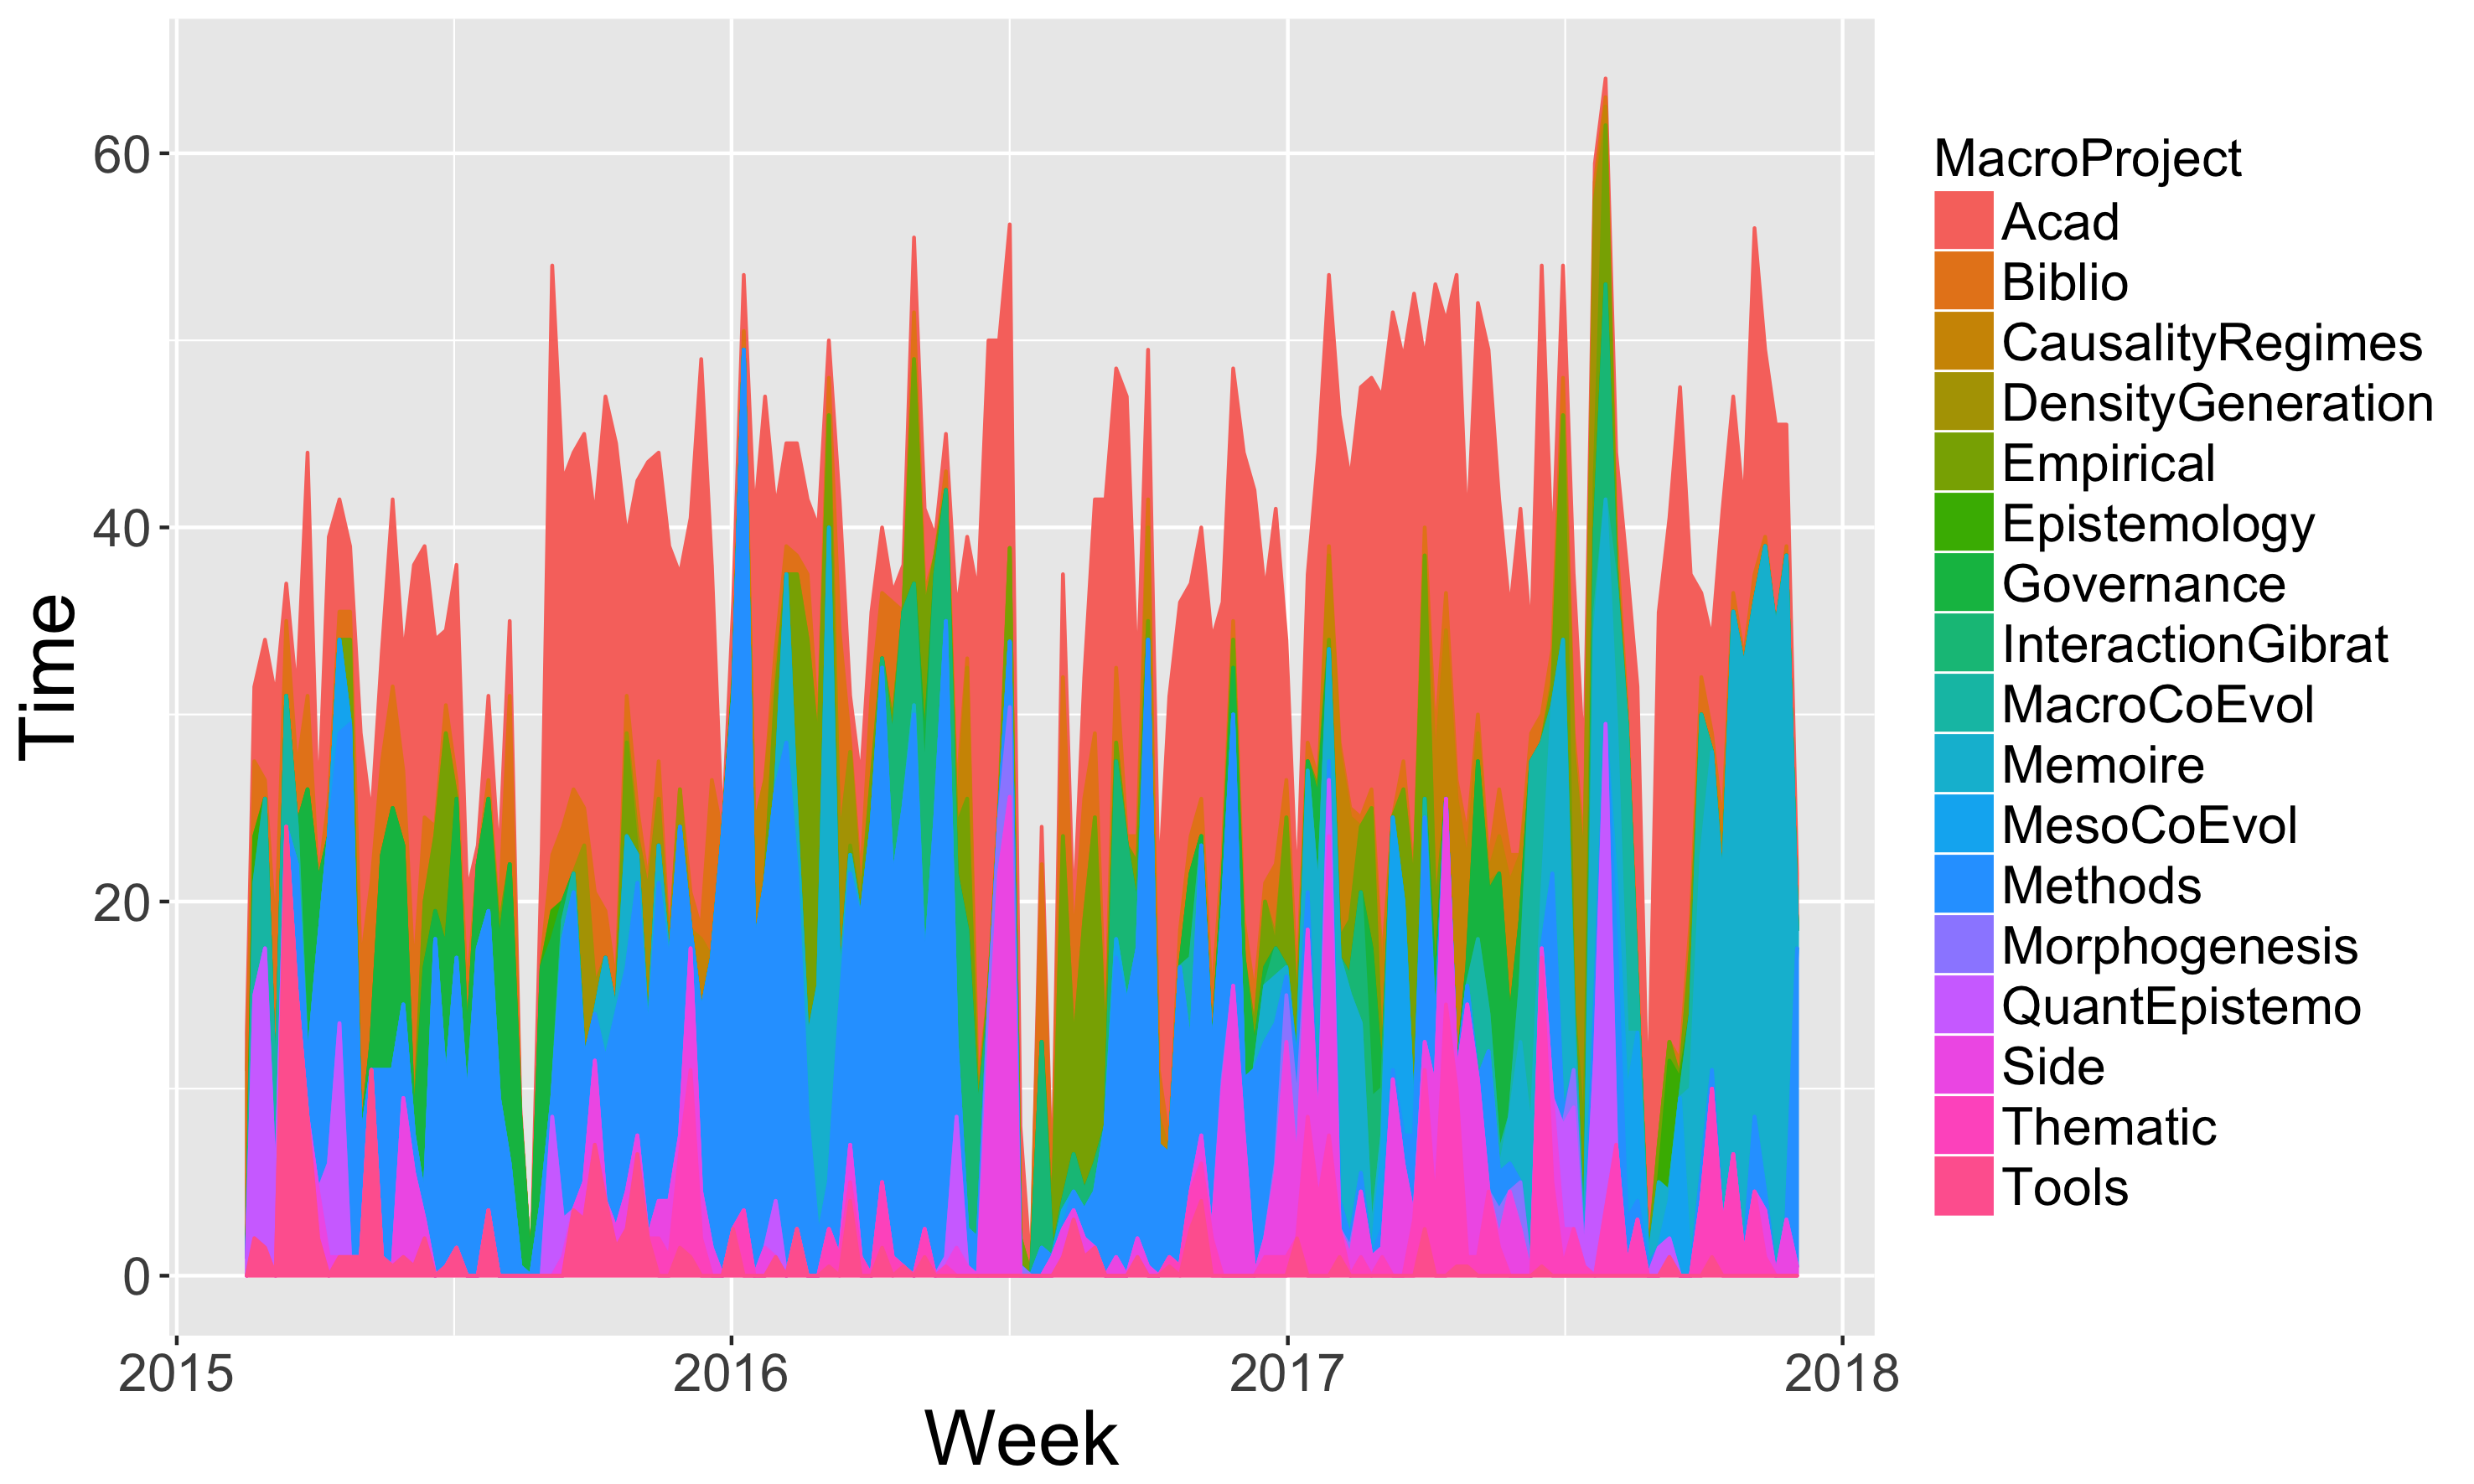
\includegraphics[width=\linewidth]{Figures/Reflexivity/weekly-macroproj.png}
	%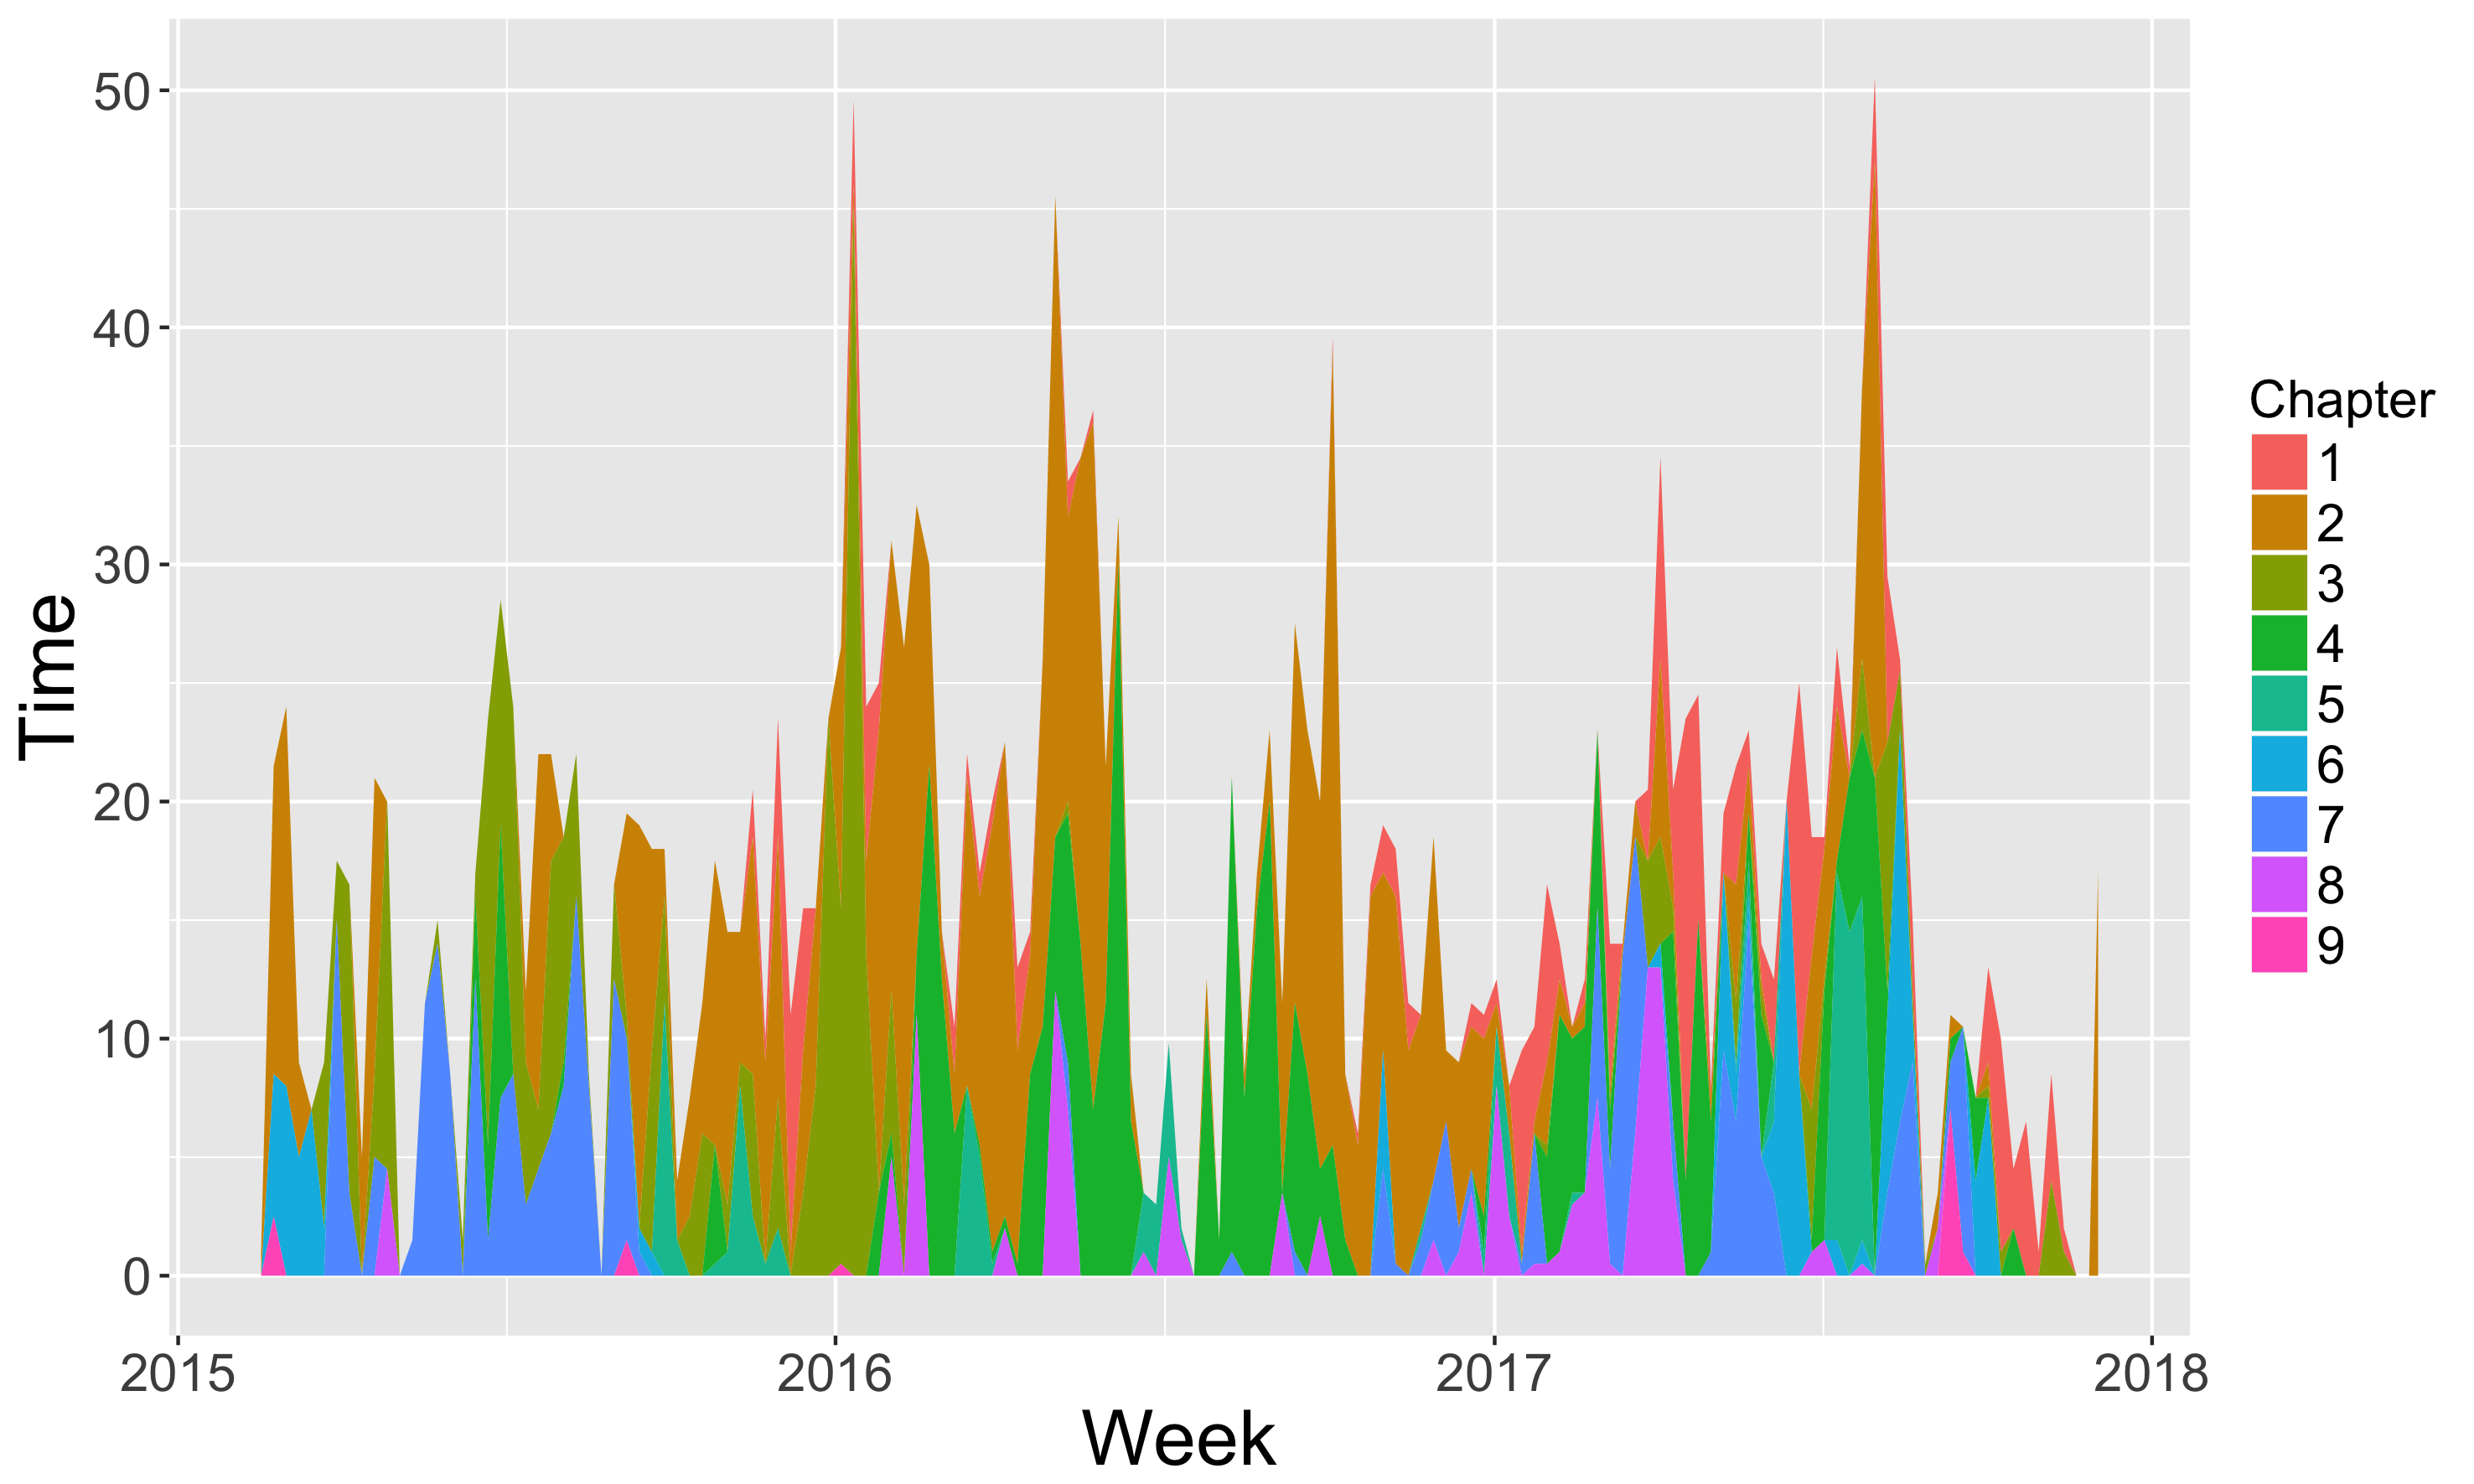
\includegraphics[width=\linewidth]{Figures/Reflexivity/weekly-chapter.png}
	%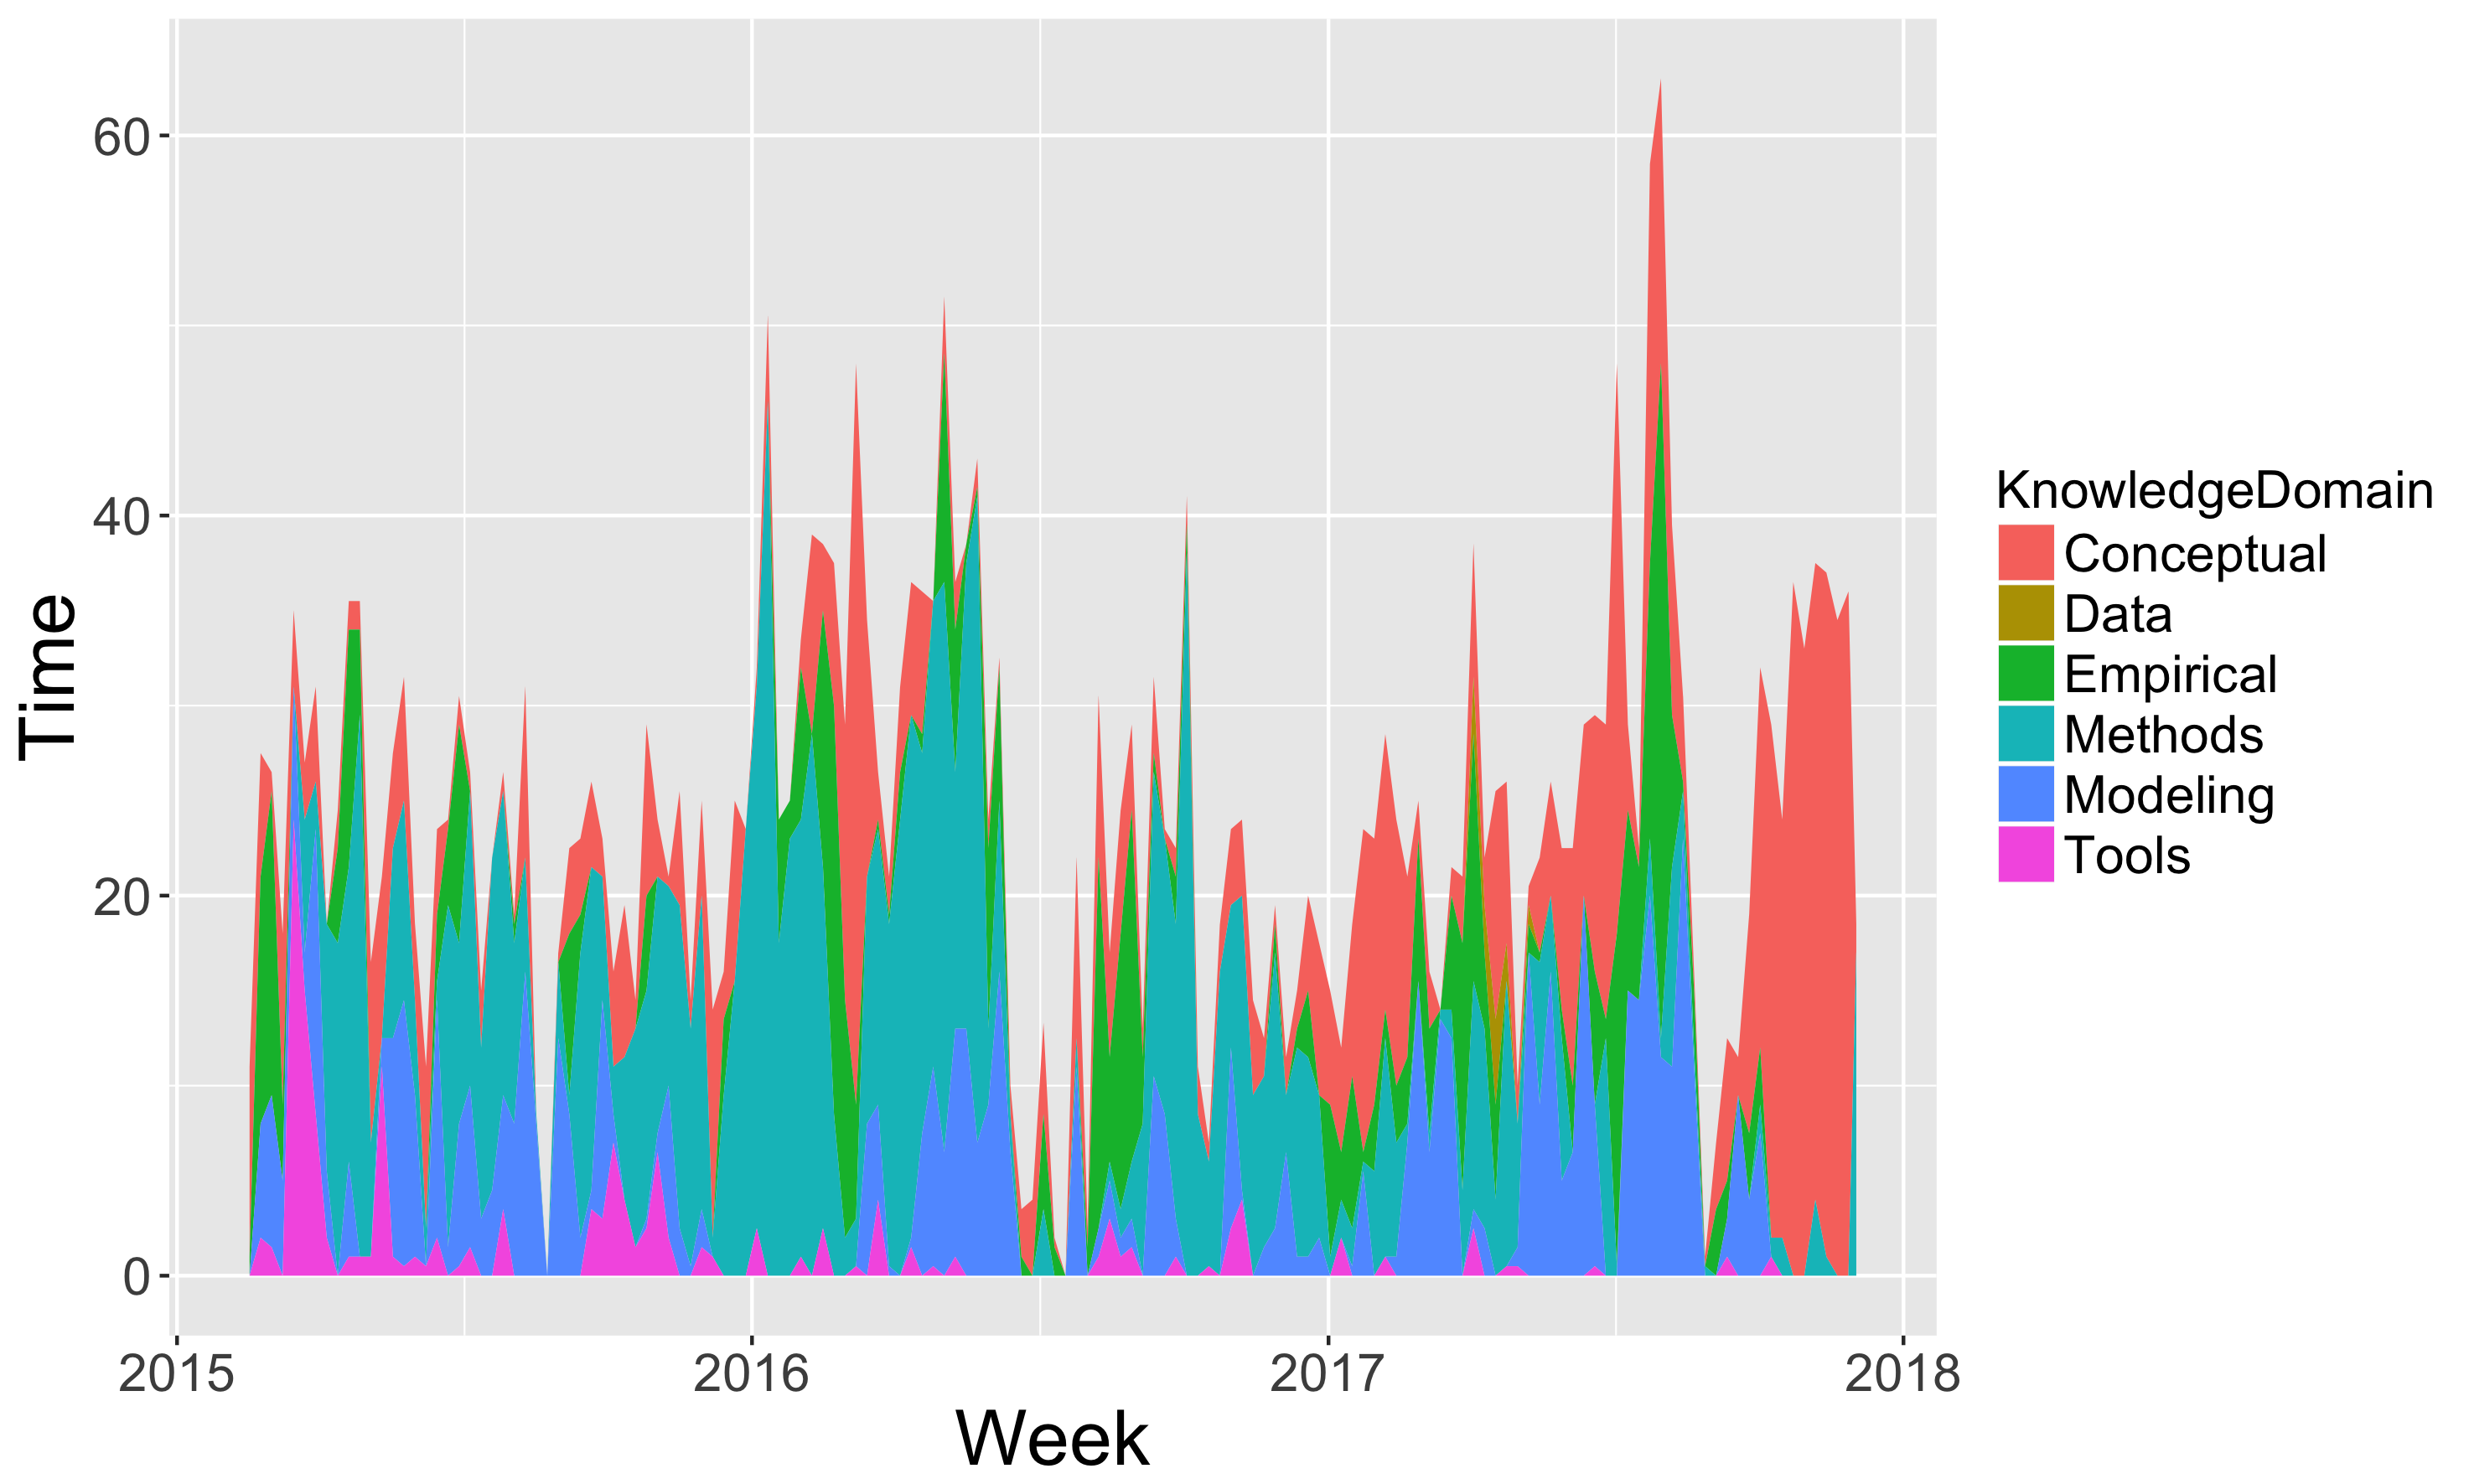
\includegraphics[width=\linewidth]{Figures/Reflexivity/weekly-knowledgedomains.png}
	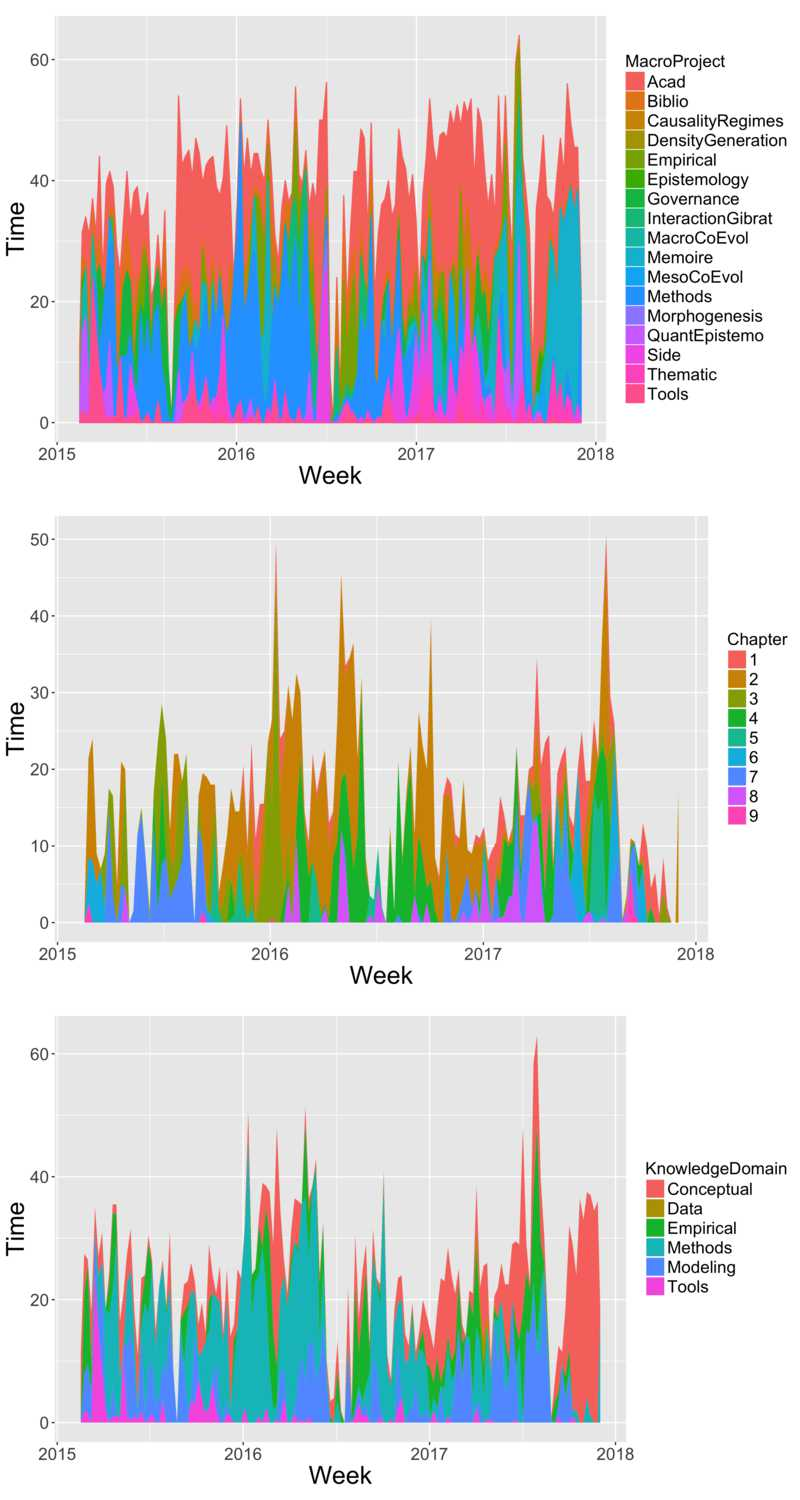
\includegraphics[width=\linewidth,height=\textheight]{Figures/Final/F-reflexivity-time.jpg}
	\appcaption{\textbf{Temporal distribution.} Times are aggregated at the level of the week and areas in color give the temporal distribution for macro-projects (\textit{first row}), chapters (\textit{second row}) and knowledge domains (\textit{third row}).\label{fig:app:reflexivity:time}}{\textbf{Répartition temporelle.} Les temps sont agrégés à la semaine et les aires en couleur donnent la répartition temporelle pour les macro-projets (\textit{première ligne}), les chapitres (\textit{deuxième ligne}) et les domaines de connaissance (\textit{troisième ligne}).\label{fig:app:reflexivity:time}}
\end{figure}
%%%%%%%%%%%%



\bpar{
It is then possible to construct interaction graphs between macro-projects or knowledge domains, assuming simplifying hypotheses.
}{
Il est possible ensuite de construire des graphes d'interaction entre macro-projets ou domaines de connaissance, moyennant des hypothèses simplificatrices.
}

\bpar{
A first index of simultaneous interaction is based on an apparition at the same time. We denote $T_{i,t}$ the time for the entity $i$ (macro-project or knowledge domain) on the temporal unit $t$ (that we take as the week). The probability of simultaneous occurrence between $i$ and $j$ is at time $t$ given by $\frac{T_{i,t}T_{j,t}}{\left(\sum_i T_{i,t}\right)^2}$, and we can sum them in time to obtain an index of interaction between entities:
}{
Un premier indice d'interaction simultanée se base sur l'apparition au même instant. Notons $T_{i,t}$ le temps pour l'entité $i$ (macro-projet ou domaine de connaissance) sur l'unité temporelle $t$ (que nous prendrons à la semaine). La probabilité d'occurrence simultanée entre $i$ et $j$ est à l'instant $t$ donnée par $\frac{T_{i,t}T_{j,t}}{\left(\sum_i T_{i,t}\right)^2}$, et nous pouvons les cumuler dans le temps pour avoir un indice d'interaction entre entités :
}
\[
I_{i,j} = \sum_t \frac{T_{i,t}T_{j,t}}{\left(\sum_i T_{i,t}\right)^2}
\]
% TODO idee : interaction croisee macroprojects - KD ?

\bpar{
The matrix $(I_{i,j})$ allows then to construct a network. A similar index based uniquely on co-occurrence is given by
}{
La matrice $(I_{i,j})$ permet alors de construire un réseau. Un indice similaire se basant uniquement sur la co-occurrence est donné par
}

\[
C_{i,j} = \sum_t \mathbbm{1}_{T_{i,t} > 0} \mathbbm{1}_{T_{j,t} > 0}
\]

\bpar{
We also look at lagged interactions, under the assumption that an entity at time $t$ can trigger the one at time $t+1$, the non-symmetrical index being then
}{
Nous regardons également des interactions retardées, sous l'hypothèse qu'une entité à l'instant $t$ puisse déclencher celle à l'instant $t+1$, l'indice non symétrique étant alors
}
\[
\tilde{I}_{i \rightarrow j} = \sum_t \frac{T_{i,t}T_{j,t+1}}{\sum_i T_{i,t}\sum_j T_{j,t+1}}
\]

\bpar{
and the same index of lagged co-occurrence
}{
et le même indice de co-occurence retardé
}

\[
\tilde{C}_{i\rightarrow j} = \sum_t \mathbbm{1}_{T_{i,t} > 0} \mathbbm{1}_{T_{j,t+1} > 0}
\]


%%%%%%%%%%%%%%%%%%
%% -- TRAD --
%%%%%%%%%%%%%%%%%%



Nous montrons les graphes correspondants pour les macro-projets en Fig.~\ref{fig:app:reflexivity:projects}. Concernant les macro-projets, il apparait que le coeur du réseau de co-occurrence simultanée est constitué par la bibliographie, la vie académique et les méthodes : ces éléments sont quasiment présent à chaque instant et structurent le reste de la recherche. Ensuite, les différents projets thématiques peuvent être menés relativement indépendamment, et gravitent à la périphérie du réseau. Avec le graphe dirigé des interactions retardées, il n'est guère possible de tirer une information supplémentaire, les flux étant quasi-symétriques : soit l'agrégation à la semaine n'est pas pertinente soit le délai peut être différent, soit il y a effectivement réciprocité, cette dernière hypothèse étant crédible vu l'intrication des projets.


%%%%%%%%%%%%
\begin{figure}
	%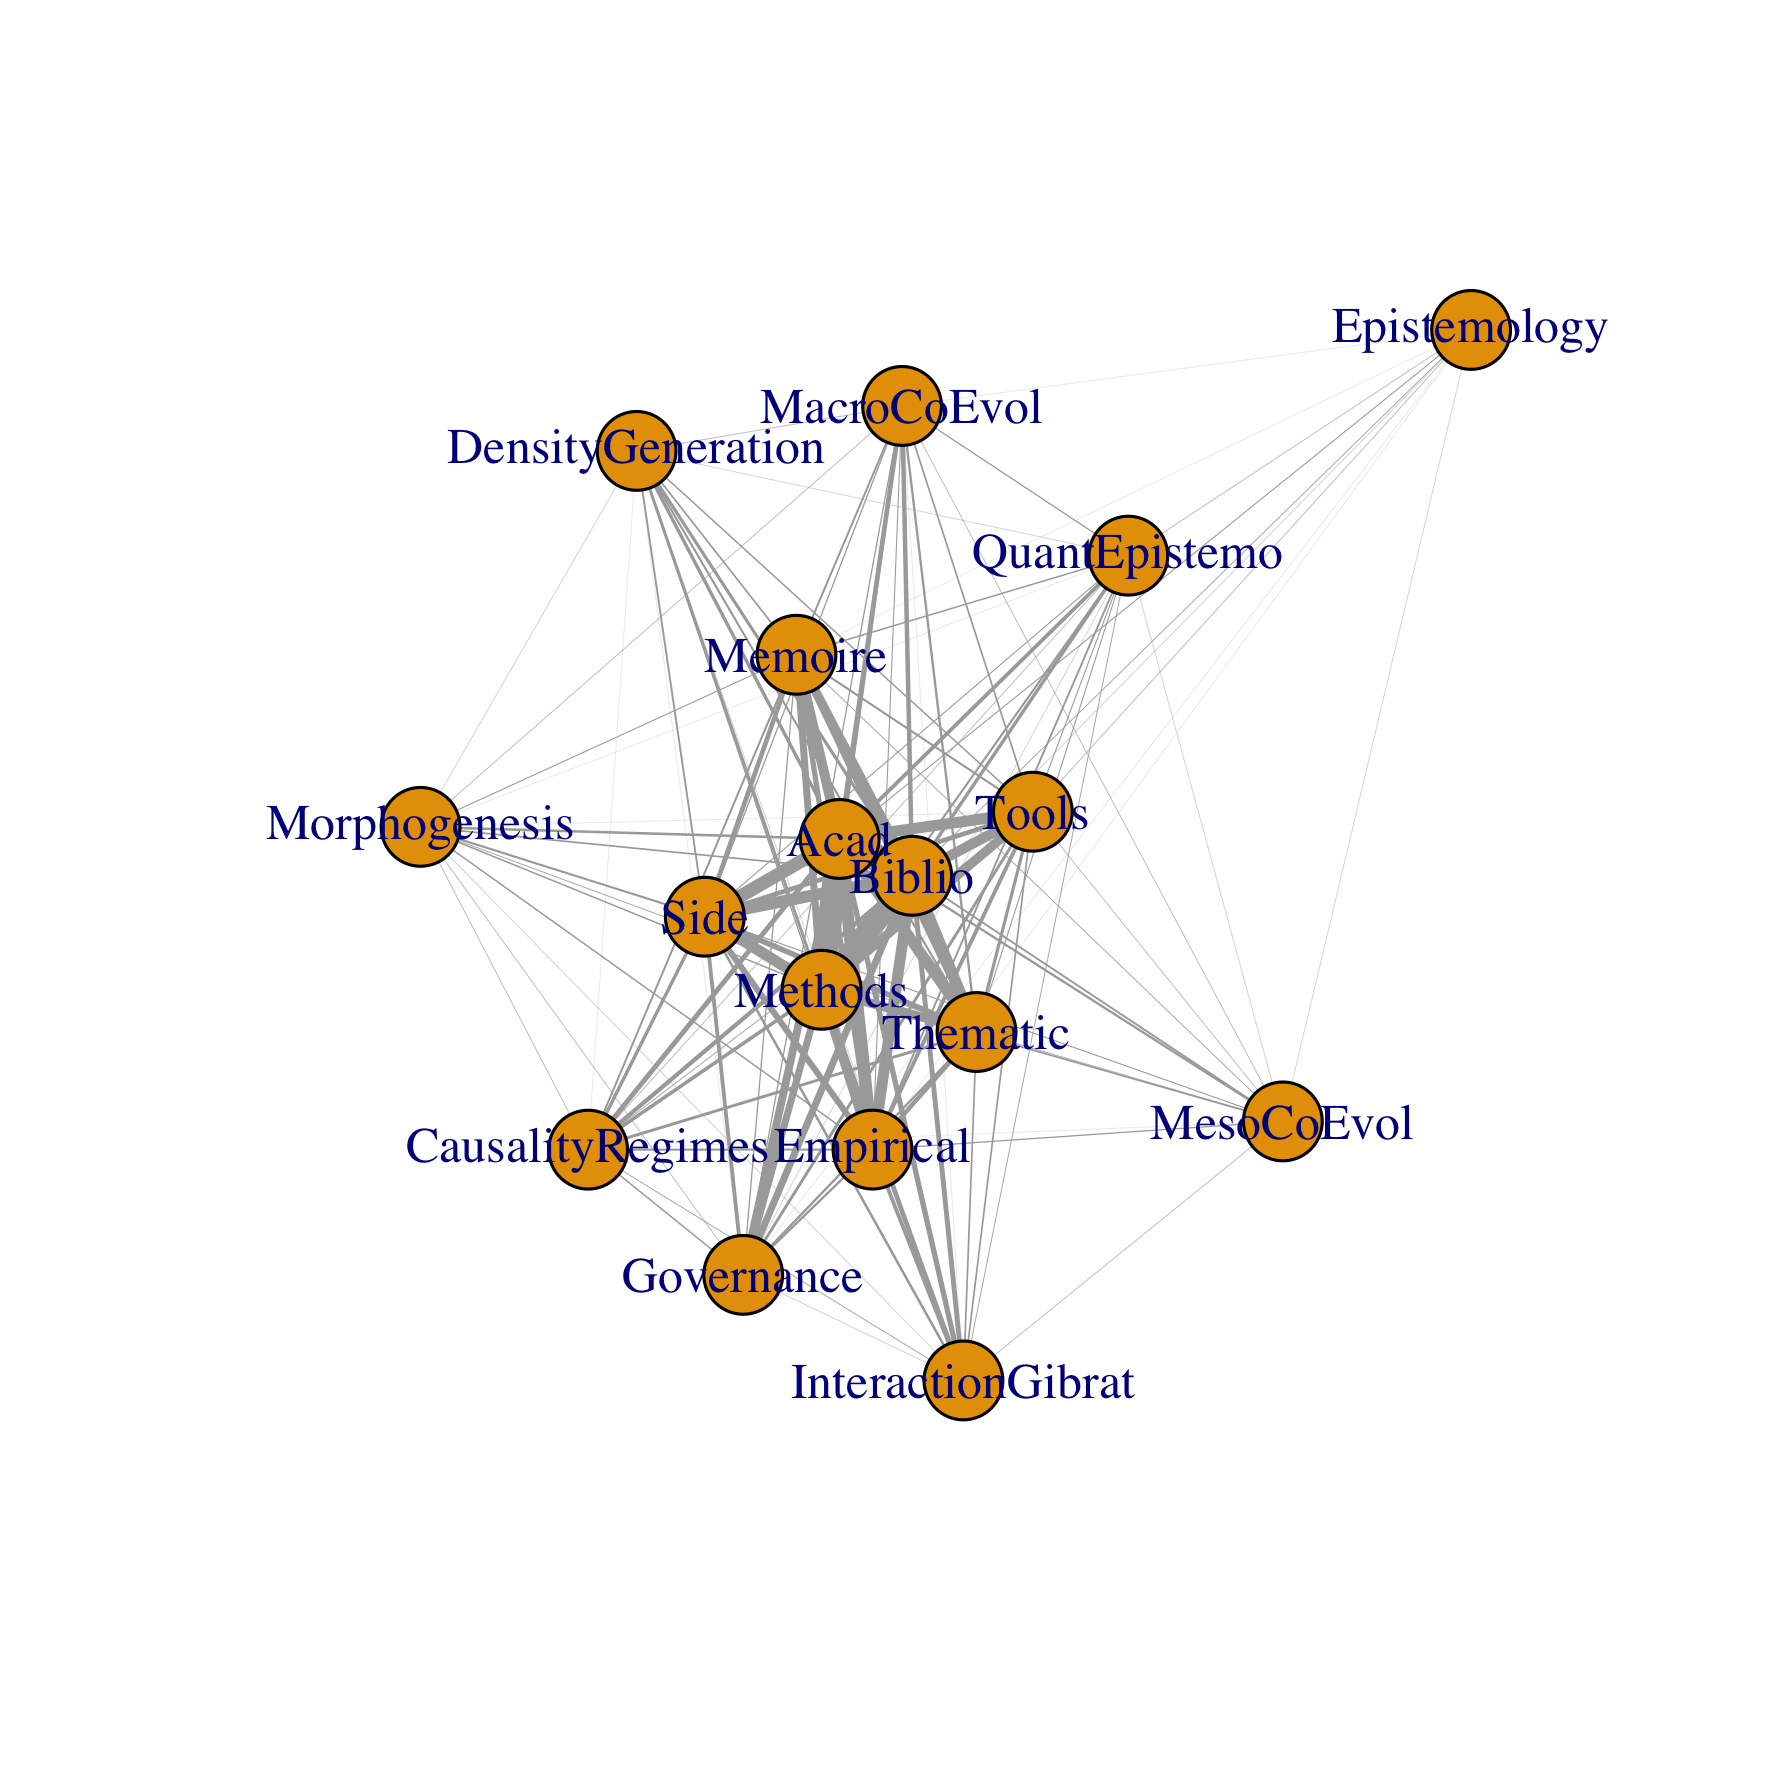
\includegraphics[width=0.49\linewidth]{Figures/Reflexivity/graph-projects-cooccs.png}
	%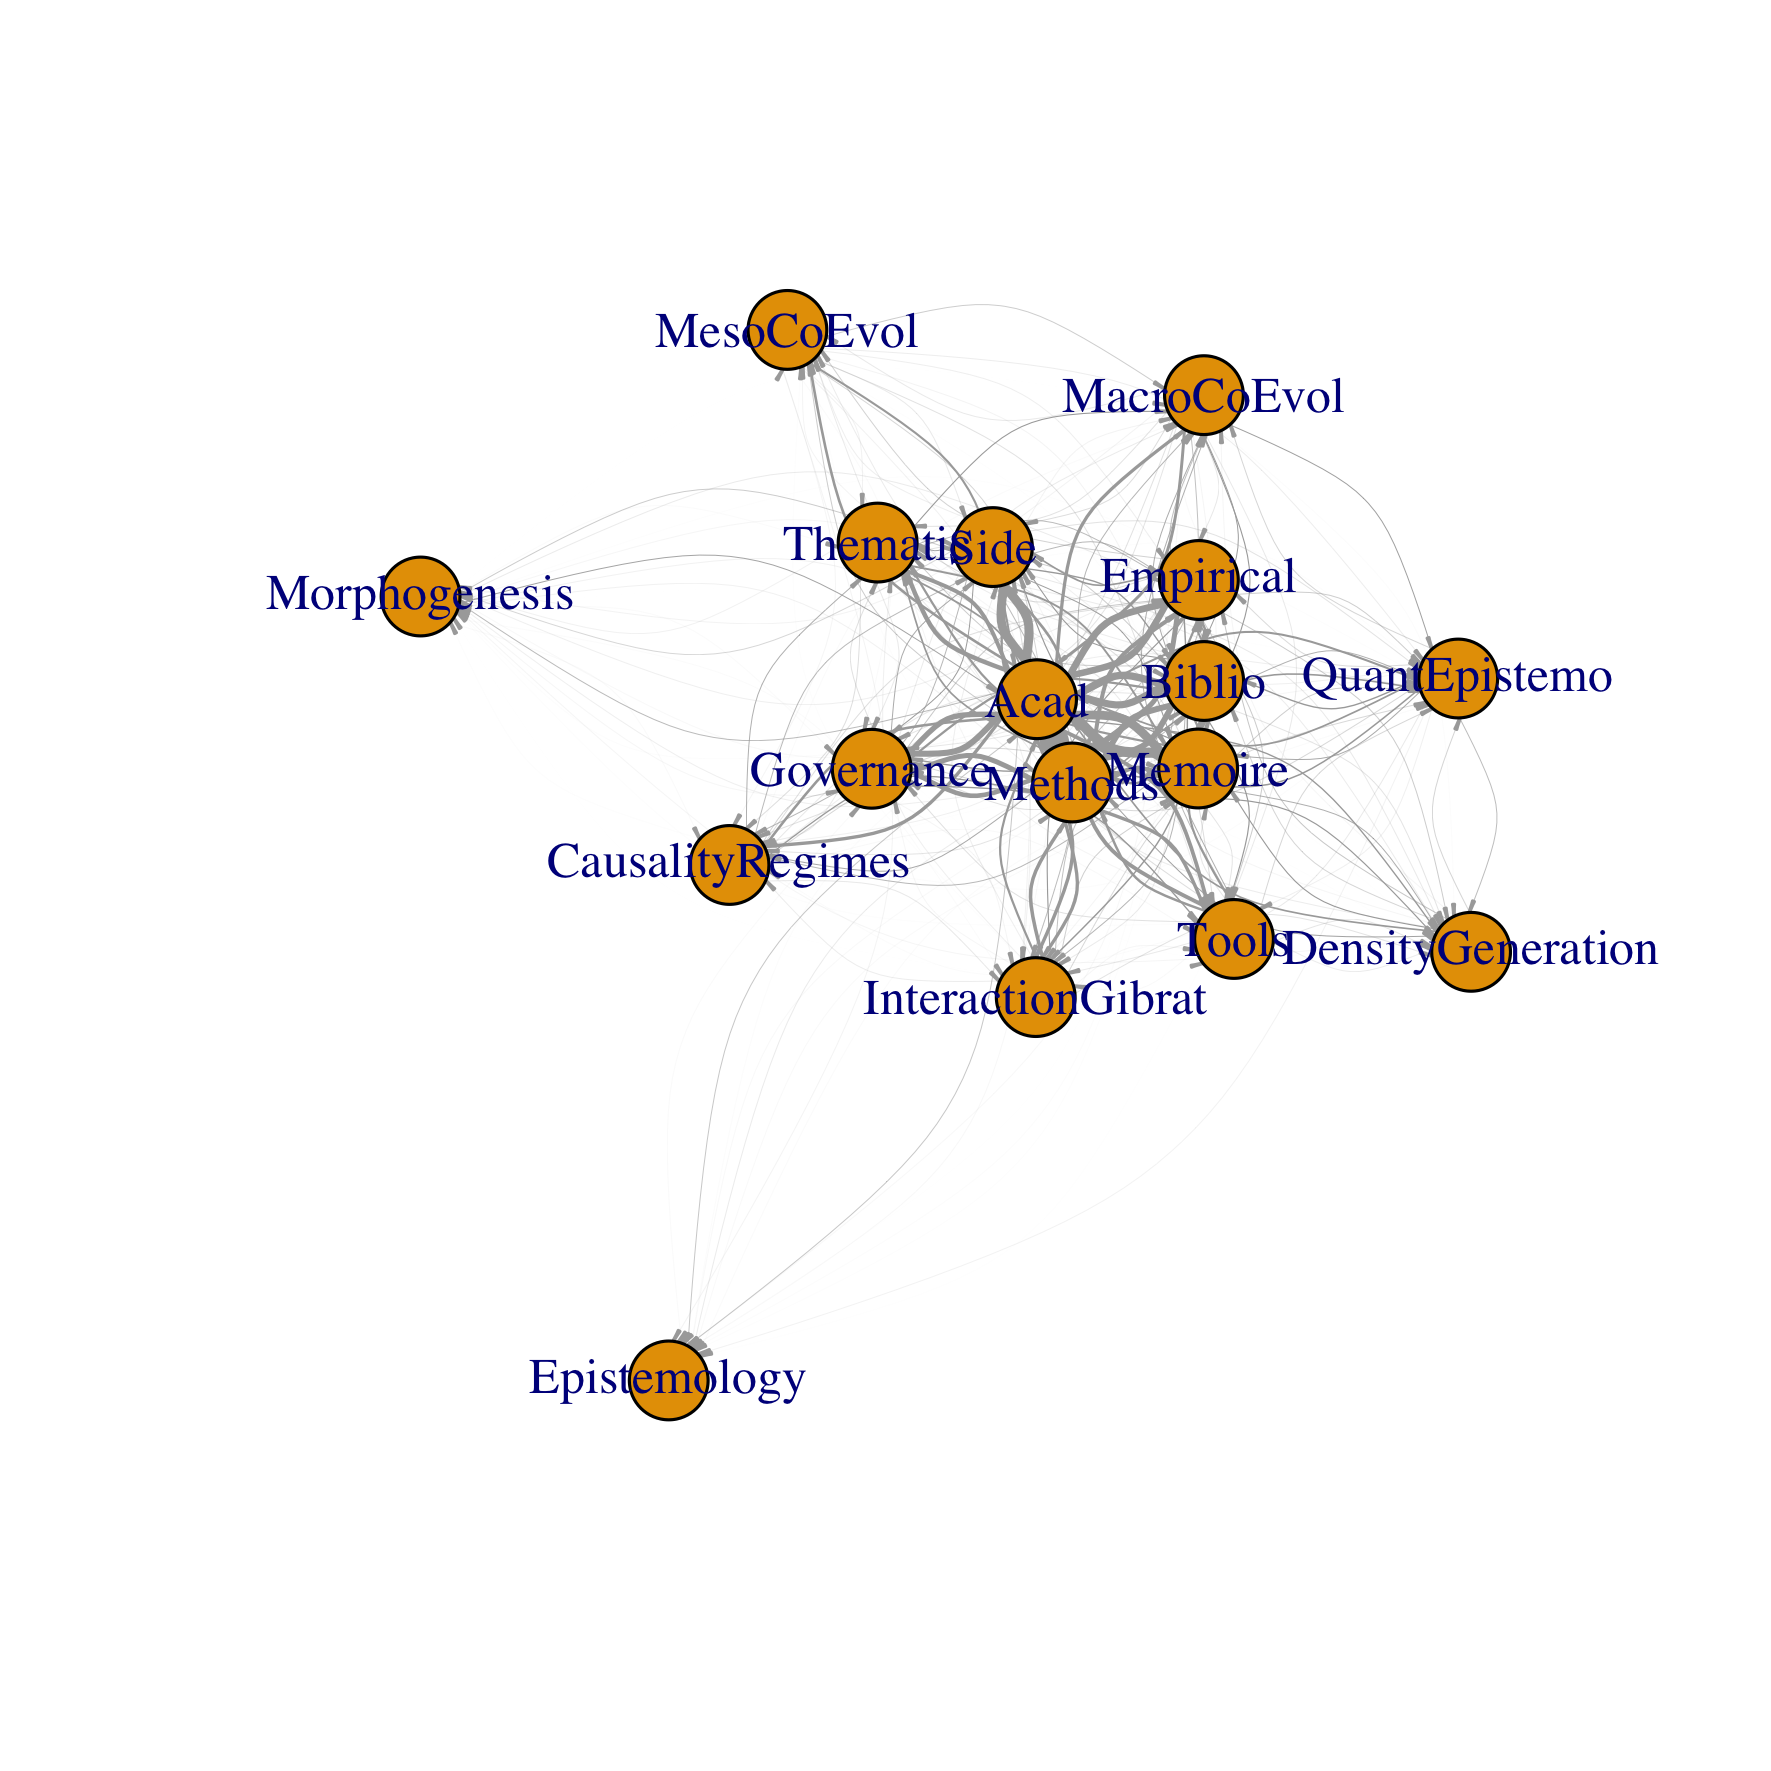
\includegraphics[width=0.49\linewidth]{Figures/Reflexivity/graph-projects-laggedflow.png}
	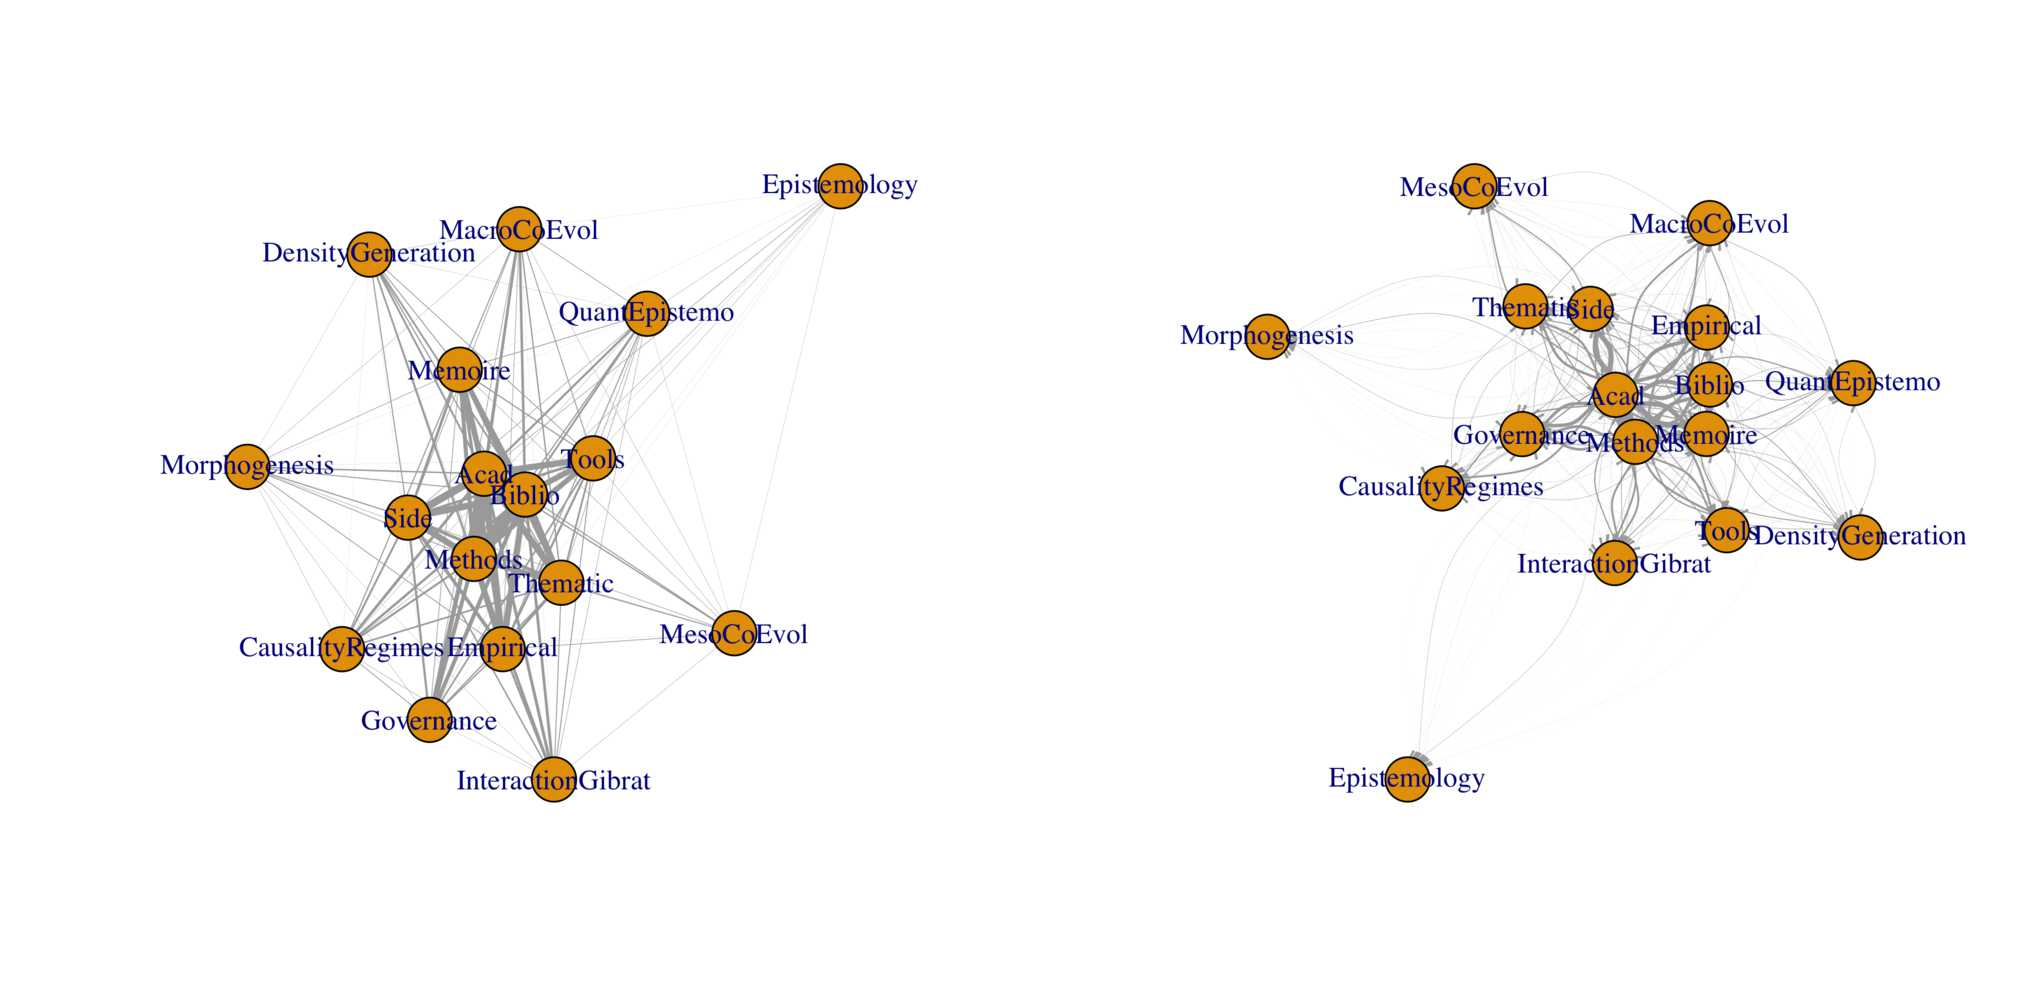
\includegraphics[width=\linewidth]{Figures/Final/F-reflexivity-projects.jpg}
	\appcaption{\textbf{Interaction networks between projects}\label{fig:app:reflexivity:projects}}{\textbf{Graphes d'interaction entre macro-projets.} (\textit{Gauche}) Graphe d'interaction simultanée par co-occurrence, donné par la matrice d'adjacence $C_{i,j}$ ; (\textit{Droite}) Graphe d'interaction retardée, donné ici par les flux $\tilde{I}_{i \rightarrow j}$. \label{fig:app:reflexivity:projects}}
\end{figure}
%%%%%%%%%%%%


Les graphes pour les domaines de connaissance est donné en Fig.~\ref{fig:app:reflexivity:kd}. Outre que les données sont relativement périphériques, ce qui est attendu vu leur faible importance et leur intégration au sein d'autres projets, nous n'observons pas de motifs particuliers dans ces graphes : l'ensemble des domaines est mobilisé à la plupart des instants. Il y a également l'ensemble des relations réciproques dans le graphe dirigé, ce qui suggère éventuellement une co-évolution entre les domaines de connaissance, ce que nous allons vérifier par la suite.

%%%%%%%%%%%%
\begin{figure}
	%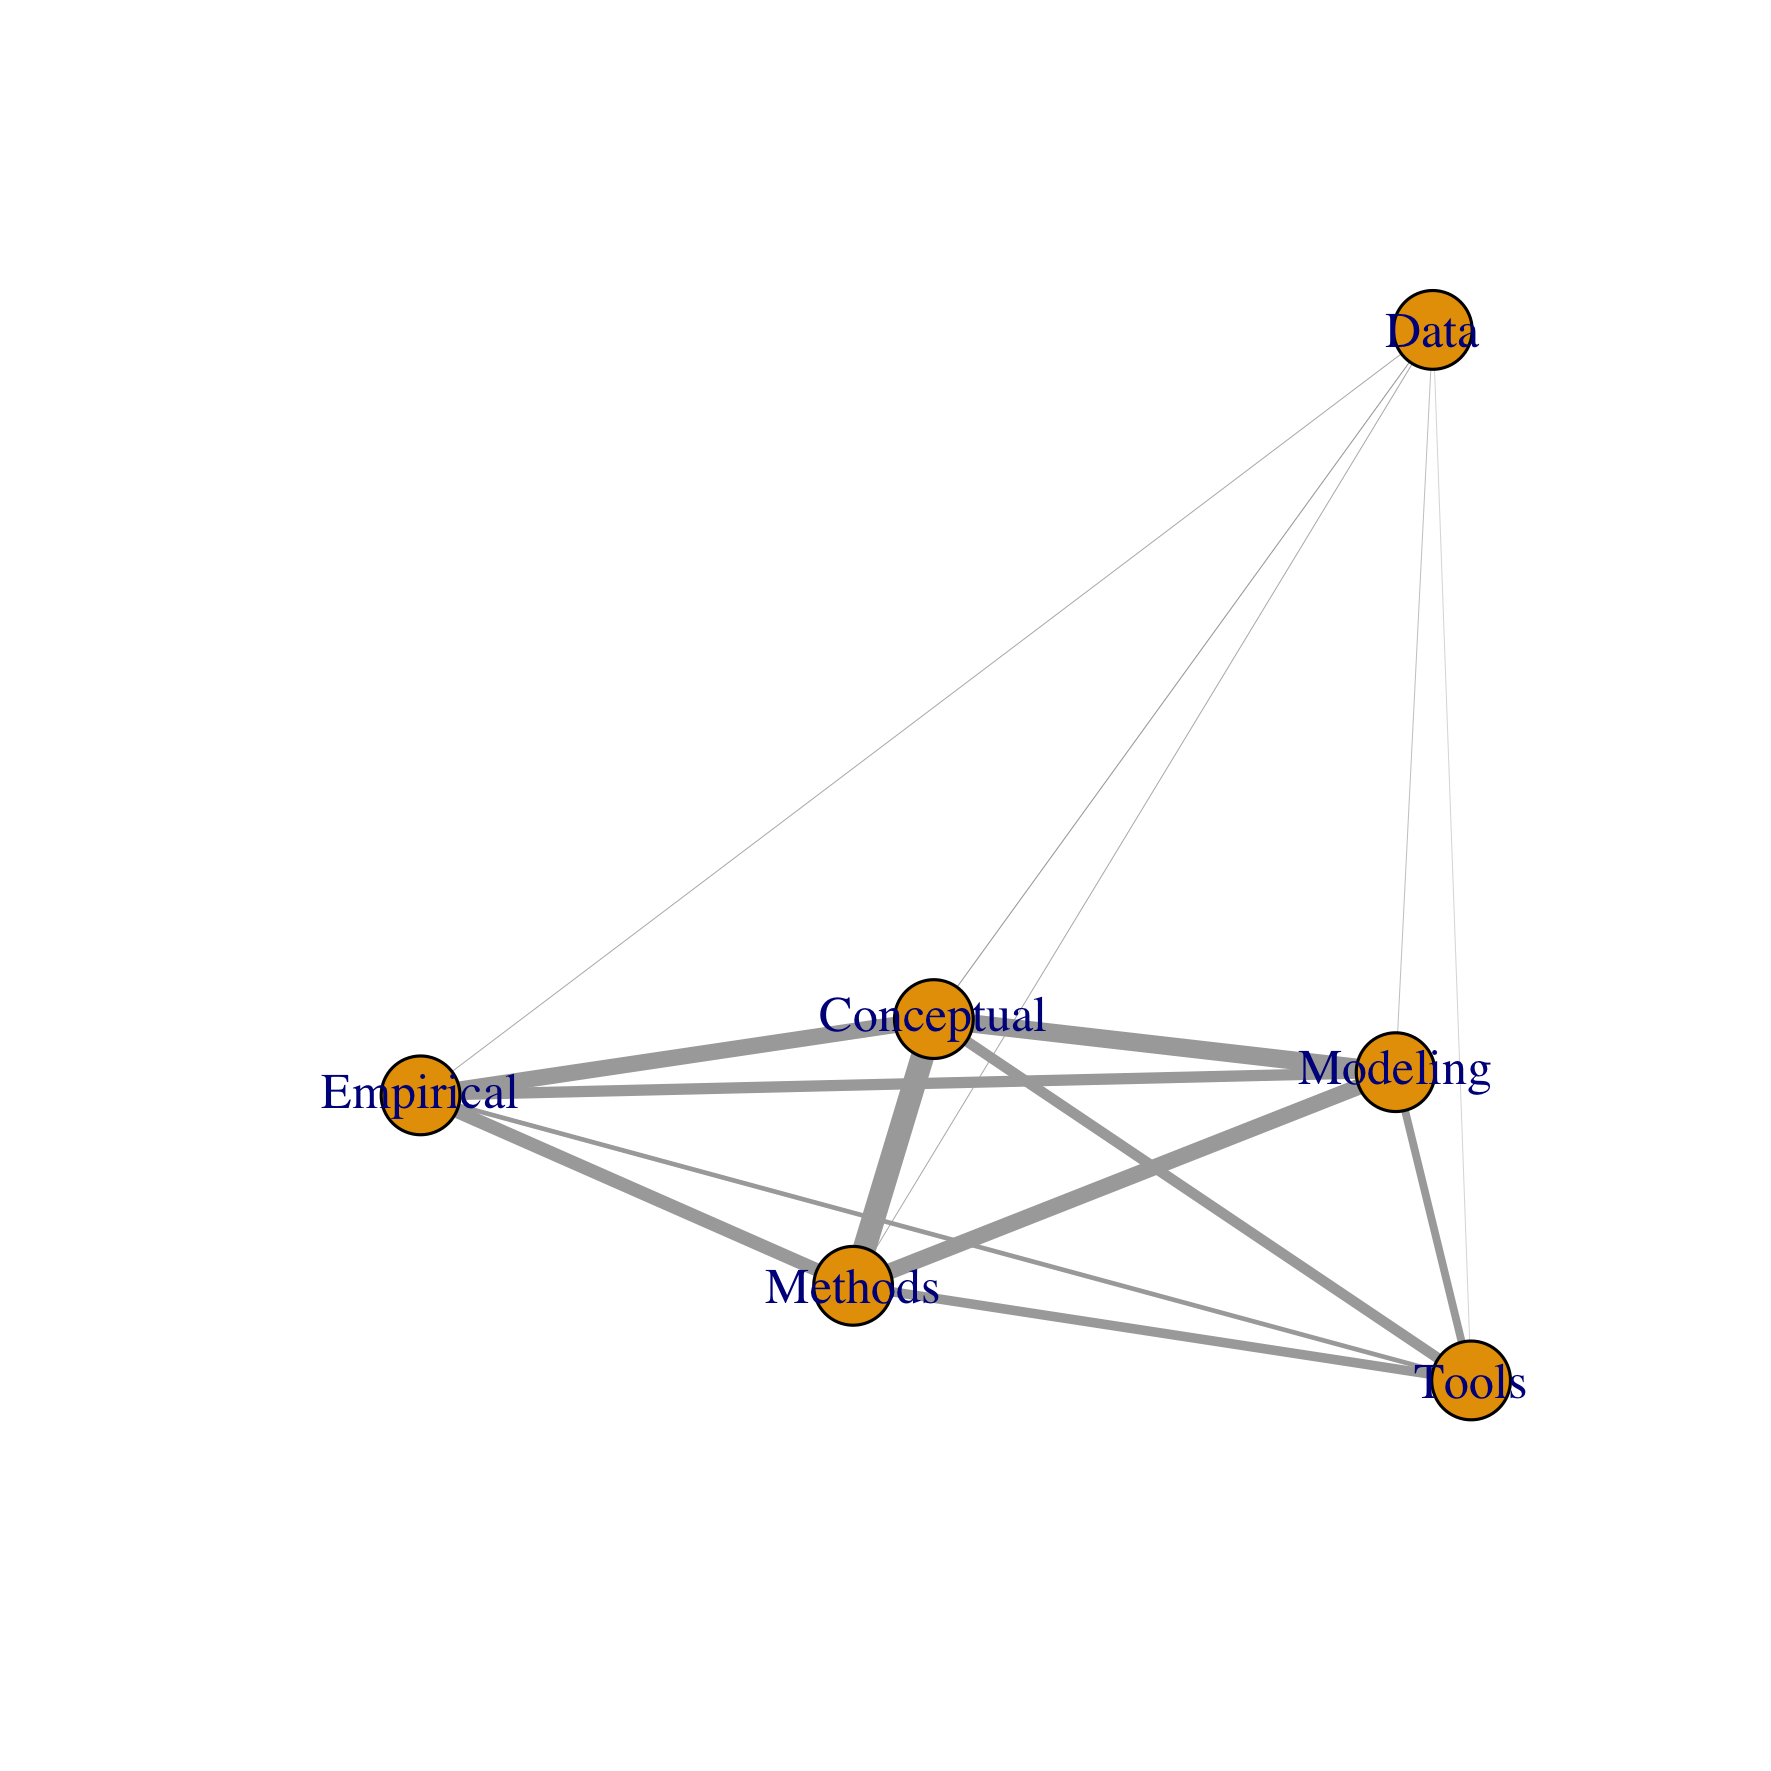
\includegraphics[width=0.49\linewidth]{Figures/Reflexivity/graph-kd-cooccs.png}
	%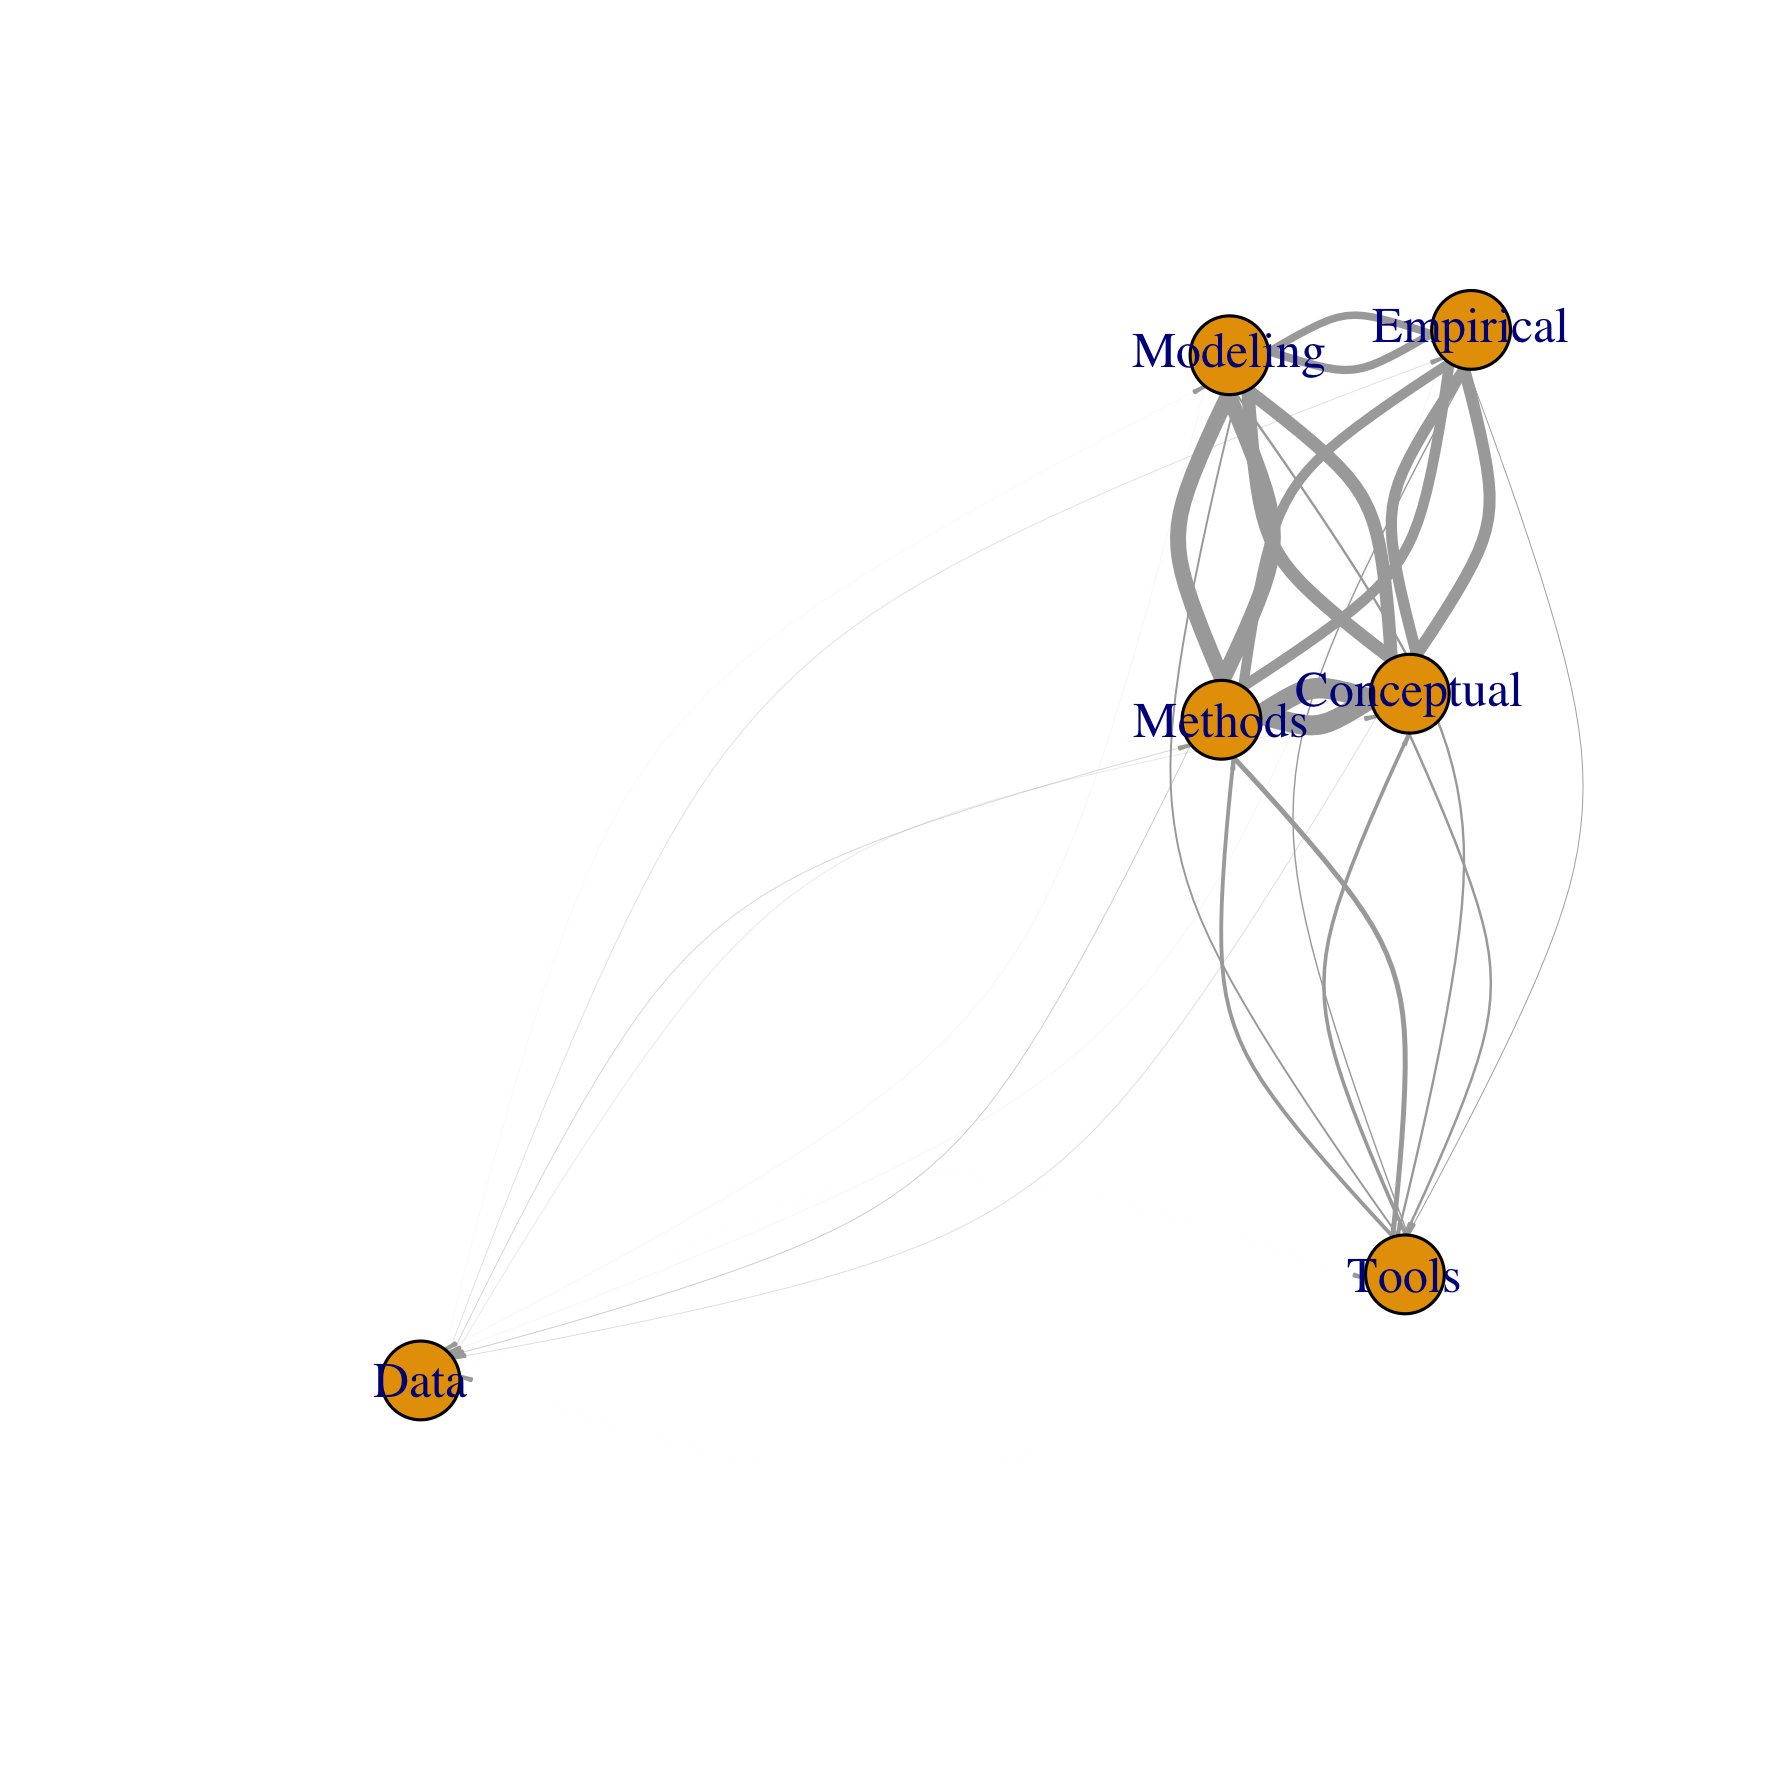
\includegraphics[width=0.49\linewidth]{Figures/Reflexivity/graph-kd-laggedflow.png}
	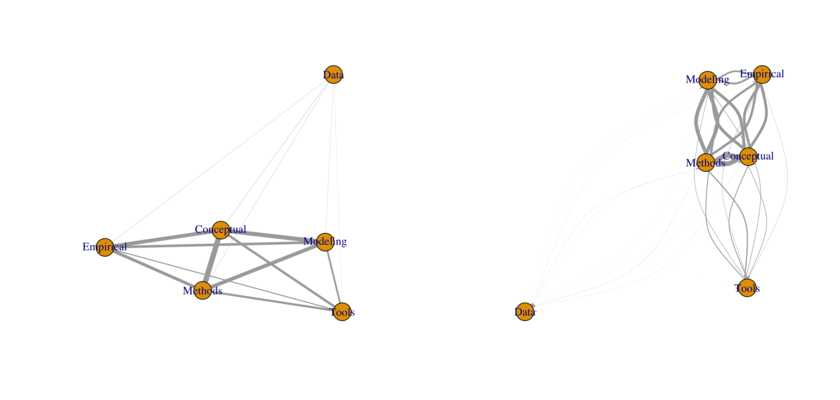
\includegraphics[width=\linewidth]{Figures/Final/F-reflexivity-kd.jpg}
	\appcaption{\textbf{Interaction networks between knowledge domains.}\label{fig:app:reflexivity:kd}}{\textbf{Graphes d'interaction entre domaines de connaissance.} (\textit{Gauche}) Graphe d'interaction simultanée par co-occurrence ; (\textit{Droite}) Graphe d'interaction retardée.\label{fig:app:reflexivity:kd}}
\end{figure}
%%%%%%%%%%%%



% kddata%>%group_by(KnowledgeDomain)%>%summarise(time=sum(time))
%  KnowledgeDomain   time
%           <fctr>  <dbl>
%1      Conceptual 1003.8
%2            Data   13.0
%3       Empirical  496.0
%4         Methods 1256.0
%5        Modeling  656.0
%6           Tools  147.0


Nous estimons pour chaque couple de domaine de connaissance $i,j$ (hors du domaine données qui ne cumule que 13h au total donc trop peu de variations pour estimer une corrélation) les corrélations retardées entre les différences $\rhob{\Delta T_{i,t-\tau}}{T_{j,t}}$ pour $-4 \leq \tau 4$ (délai maximal d'un mois). Nous conservons les corrélations si $p<0.05$ et sélectionnons la corrélation absolue maximale pour chaque couple de variable si elle existe.

%%%%%%%%%%%%%%
\begin{figure}
	%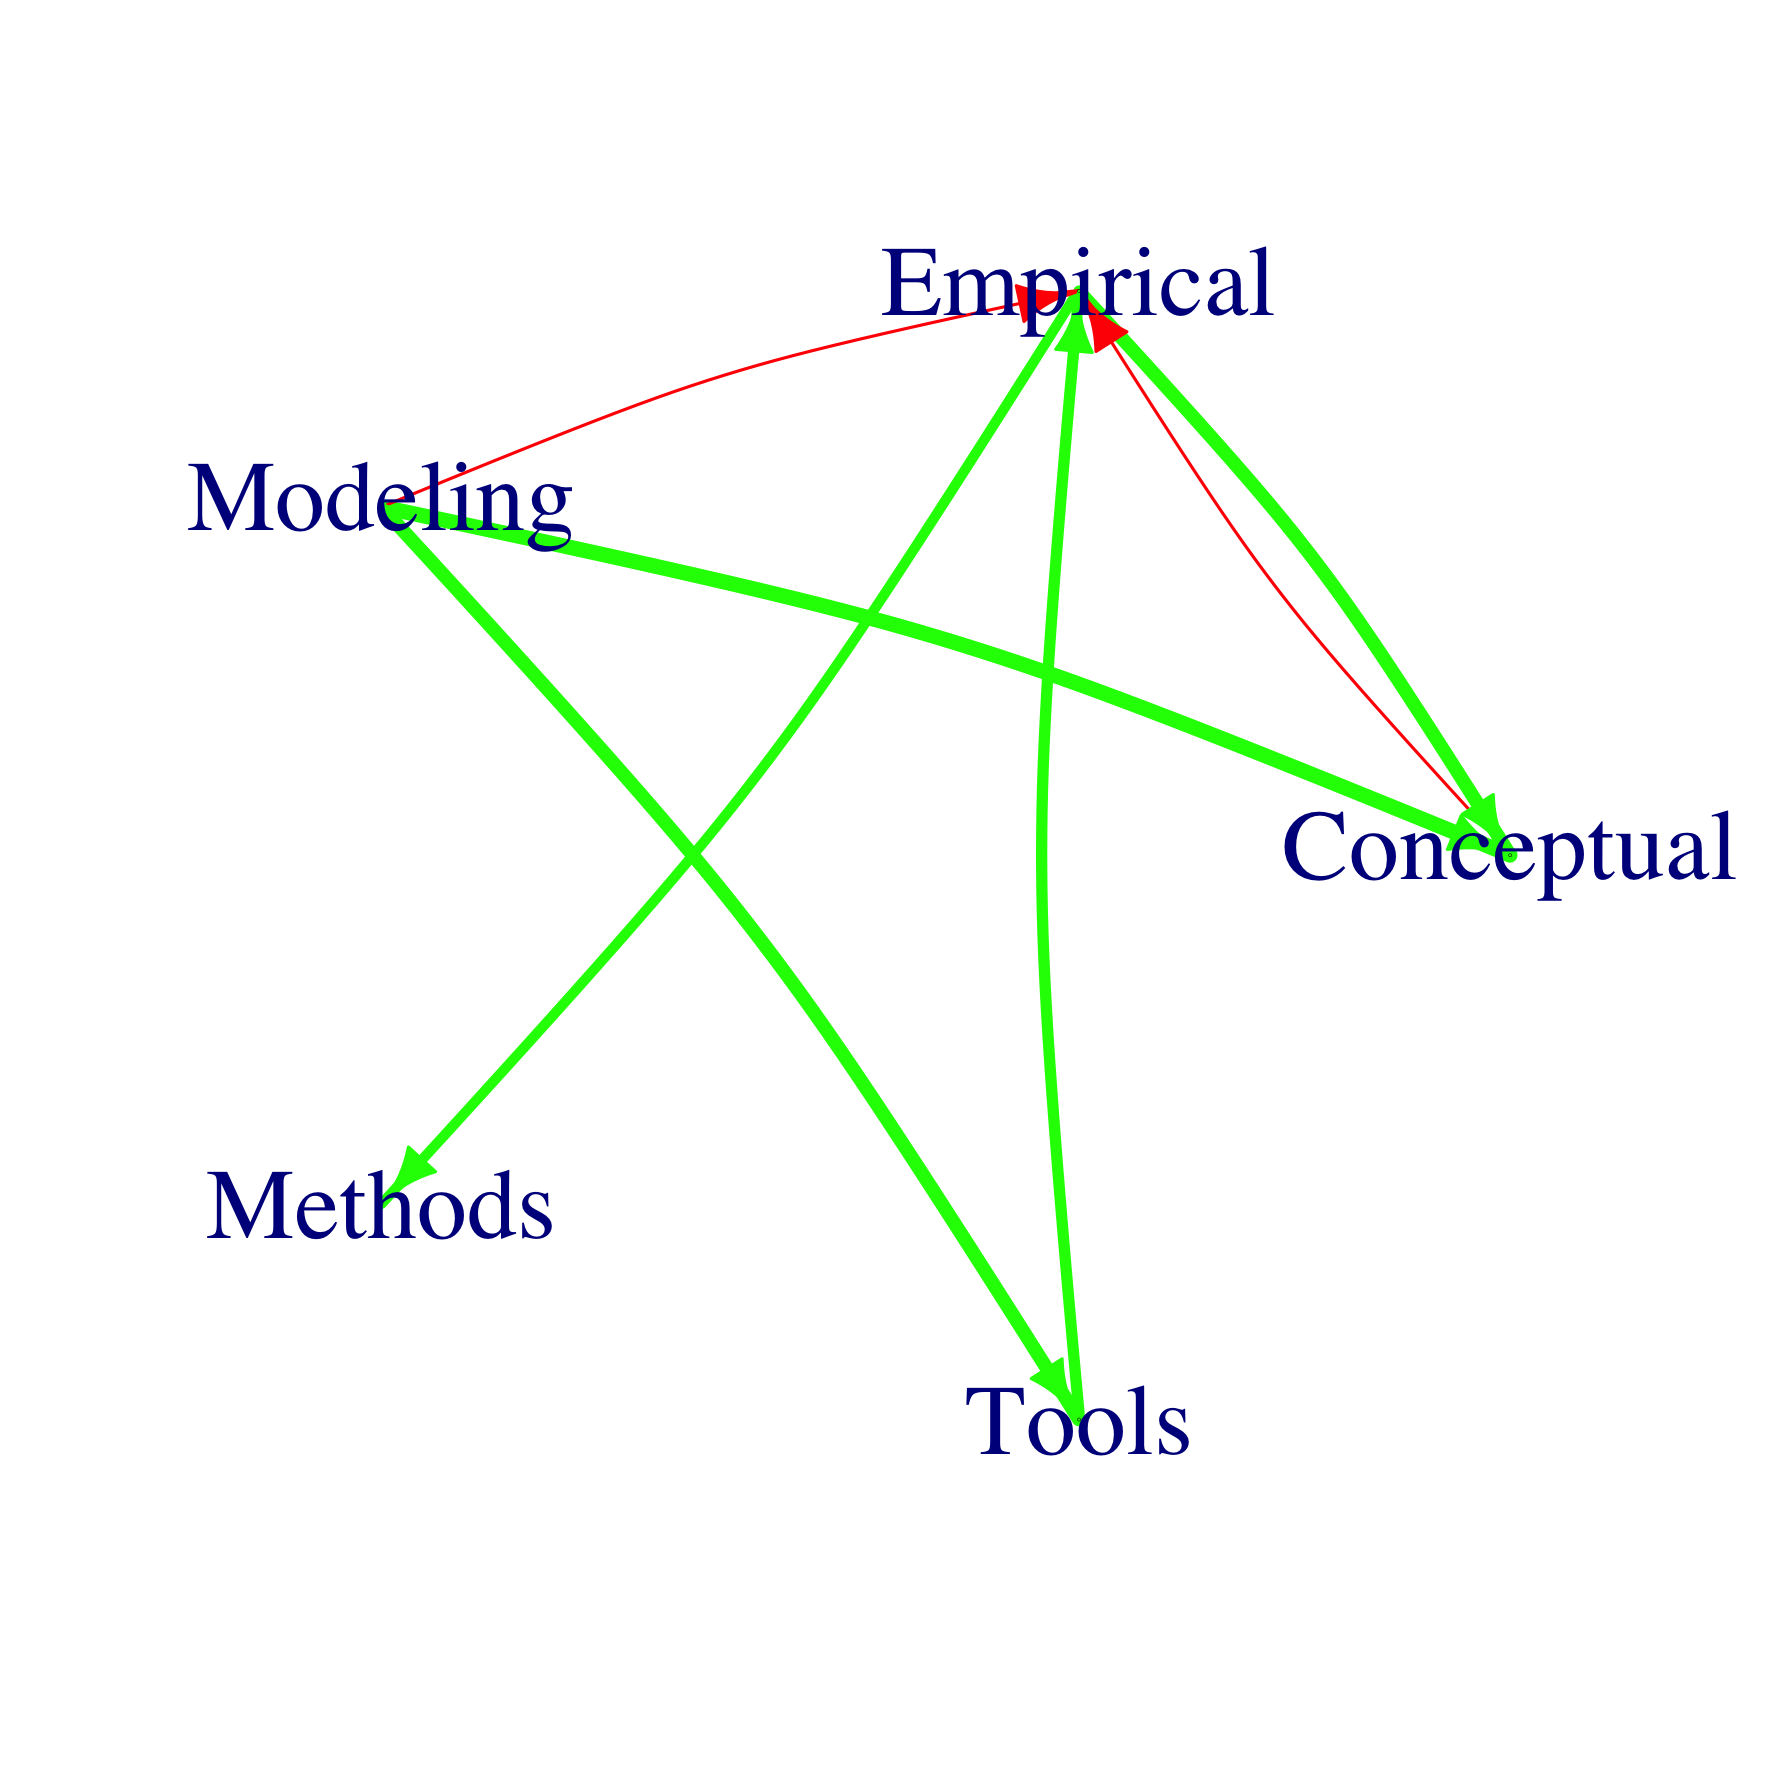
\includegraphics[width=\linewidth]{Figures/Reflexivity/laggedcorrs.png}
	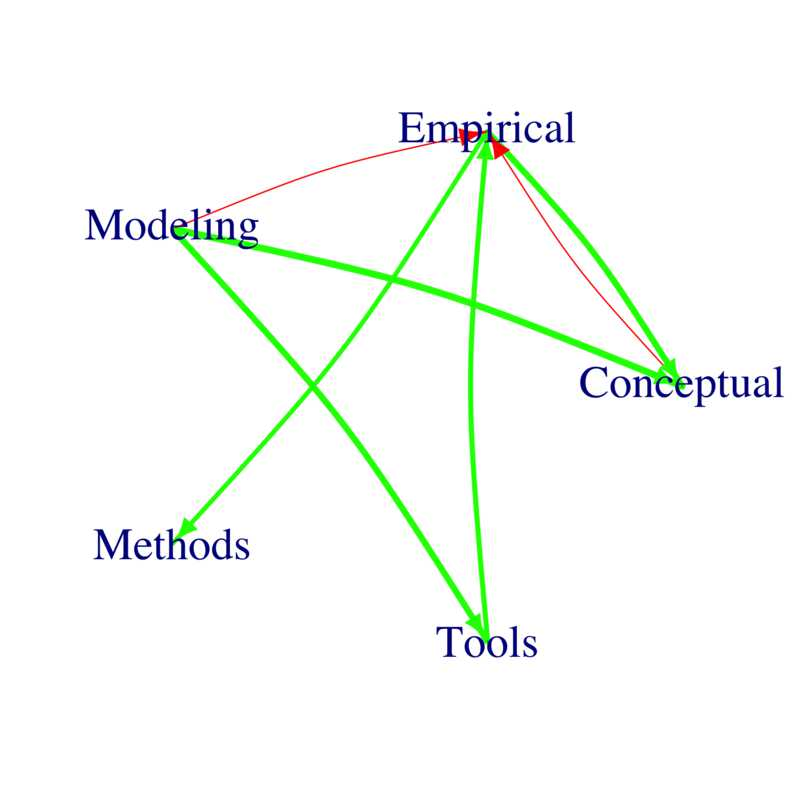
\includegraphics[width=\linewidth]{Figures/Final/F-reflexivity-laggedcorrs.jpg}
	\appcaption{\label{fig:app:reflexivity:laggedcorrs}}{\textbf{Graphe de corrélations retardées entre domaines de connaissances.} La couleur donne le signe de la corrélation (vert : positif, rouge : négatif) et l'épaisseur du lien sa valeur. Les liens existent si et seulement si $p<0.05$ pour un test de Fisher.\label{fig:app:reflexivity:laggedcorrs}}
\end{figure}
%%%%%%%%%%%%%%


Le graphe des corrélations retardées est donné en Fig.~\ref{fig:app:reflexivity:laggedcorrs}. Il existe un certain nombre de liens significatifs, et même une relation circulaire entre empirique et conceptuel, c'est-à-dire une co-évolution à proprement parler entre ces domaines. La modélisation et l'empirique induisent des travaux dans le domaine conceptuel, ce qui peut s'interpréter comme une induction des théories. Par contre, le conceptuel diminue l'empirique, ce qui pourrait être symptôme d'une trop grande déconnexion avec le concret parfois.

Ainsi, même si ces résultats sont bien sûr à prendre avec précaution vu les biais intrinsèques aux données (difficulté de donner un label, réduction au sein de projets, etc.), nous suggérons une intrication des domaines de connaissance et une co-évolution pour certains. Cela peut être mis en écho avec l'hypothèse fondamentale du cadre de connaissance développé en~\ref{sec:knowledgeframework}, qui implique qu'une connaissance complexe nécessite co-évolution des domaines. Enfin, l'application des propres outils de notre travail à lui-même suggère une dimension hologrammatique~\cite{morin1986methode}, rappelant le lien entre complexité et production de connaissance suggéré en~\ref{sec:epistemology}. 



\stars



%%%%%%%
%% -- on hold --

%%%%%%%%%%%%
%\subsection{Concept maps}{Cartographie des concepts}

%concept maps : \cite{novak2008theory}

% faire un graphe des concepts ; compare to semantic network of concepts in Gödel Escher Bach.




% To clarify the plan : Plan (of course) ; diagram for plan ; and dependence tree for parts/sections
% --> en intro


%  ``Meta-conclusion''
%  -> should also include reading graph / possible paths





